\documentclass[11pt,titlepage]{article}

\usepackage{packages}
\addbibresource{bib/Biblio.bib}
\selectlanguage{french}

\begin{document}
\renewcommand{\headrulewidth}{0pt}

\pagestyle{fancy}
%... then configure it.
\fancyhead{} % clear all header fields
\fancyhead[L]{École Nationale des Ponts et Chaussées - Projet de Fin d'Études}
\fancyfoot{} % clear all footer fields
\fancyfoot[R]{\thepage}
\fancyfoot[L]{ROUDNINSKI Samuel - Département Génie Civil et Construction}

\begin{titlepage}
\center
\includegraphics[scale=0.5]{img/logo/logo_enpc.png}
\\[0.25cm]
{\large 2024}
\\[0.75cm]
{\LARGE \bfseries Projet de Fin d'Etudes}
\\[1cm]
{\Large Département Génie Civil et Construction}
\\[1cm]
{\Large Samuel ROUDNINSKI}
\\[0.5cm]
{\Large Élève ingénieur, double-diplôme d'architecture}
\\[1cm]
{\Large Tuteur professionnel: Robert Jan VAN SANTEN}
\\[1cm]
{\Large Tuteur académique: Jorge HIDALGO}
\\[1cm]
{\huge \bfseries Titre du rapport}
\\[1cm]
{\Large Rapport non confidentiel}
\\[1.5cm]
{ Stage réalisé au sein de VS-A.HK}
\\[0.25cm]
{W2, 9/F, 93 Bedford Road, Tai Kok Tsui, Kowloon, Hong Kong SAR, China}
\\[0.25cm]
{ 18 mars 2024 - 18 septembre 2024}
\end{titlepage}

\def\abstract{
   \vfil
\begin{center}%
{\bfseries \abstractname\vspace{-.5em}}%
\end{center}
\quotation
}

\def\endabstract{\par
\endquotation
}
\newpage
 
\section*{Remerciements}


\newpage
 
\section*{Résumé}

Insérez votre résumé en français.
Le résumé comprend 3 parties (contexte, missions et objectifs, résumé). L’ensemble doit faire 2600 signes maximum en comptant les espaces. La partie ‘résumé’ doit être plus longue que les 2 parties précédentes.
N’oubliez pas d’effacer ce texte quand vous n’en aurez plus besoin.

Mots-clés : 5 mots-clés

\newpage
 
\section*{Abstract}
Insérez votre résumé en anglais.
Le résumé comprend 3 parties (context, missions and goals, abstract). L’ensemble doit faire 2600 signes maximum en comptant les espaces. La partie ‘résumé’ doit être plus longue que les 2 parties précédentes.
Vous pouvez corriger votre abstract en anglais avec Writefull ou Grammarly.
N’oubliez pas d’effacer ce texte quand vous n’en aurez plus besoin.

Keywords: 5 keywords

\newpage

\renewcommand{\baselinestretch}{1.0}\normalsize
\tableofcontents
\renewcommand{\baselinestretch}{1.15}\normalsize

\newpage
 
\listoffigures
\newpage
 
\listoftables
\newpage

\newacronym{vec}{VEC}{Vitrages extérieurs collés}
\newacronym{cstb}{CSTB}{Centre Scientifique et Technique du Bâtiment}
\newacronym{dtu}{DTU}{Document Technique Unifié}
\newacronym{pvb}{PVB}{Polybutyral vinylique (feuille intercalaire liant plusieurs couches de verre entre elles dans un vitrage feuilleté)}
\newacronym{sgp}{SGP}{SentryGlas® interlayer (feuille intercalaire liant plusieurs couches de verre entre elles dans un vitrage feuilleté)}
\newacronym{FEM}{FEM}{Finite Element Method (Méthode des éléments finis)}
\newacronym{ELU}{ELU}{État Limite Ultime}
\newacronym{ELS}{ELS}{État Limite de Service}

\printglossary[type=\acronymtype,title=Liste des abréviations]
\newpage
\section{Introduction}

\subsection{Contexte}

L'expérience acquise par le bureau d'études façades VS-A sur des projets passés construits, comme les serres de Coutevroult, le quai Ouest à Boulogne Billancourt ou la Médiathèque Alexis de Tocqueville à Caen, ou théoriques, leur ont permis de démontrer le potentiel rarement exploité des vitrages plans et surtout non plans, c'est-à-dire déformés à chaud ou à froid. Ces procédés sont souvent ignorés tant par les fournisseurs de verre que par la réglementation française.

Réfléchir à des solutions pour réduire la quantité de verre des vitrages est un enjeu à la fois économique et environnemental mais également architectural, particulièrement dans le cas où l'on souhaiterait réaliser de grandes étendues vitrées transparentes puisque la transparence du verre est limitée par son épaisseur. C'est donc un défi à la fois d'ingénieur mais également d'architecte.

\subsection{Problématique et objectifs}

Ce projet de fin d'études propose de réfléchir à des solutions de verres non plans qui garantissent des performances équivalentes tout en réduisant la quantité de verre utilisée.
\\

L'objectif de ce mémoire est de mettre au point des solutions de verres autoportants, c'est-à-dire maintenus seulement en pied et en tête du vitrage, permettant de réduire la quantité de verre utilisée pour couvrir une même surface de façade, tout en garantissant les mêmes performances qu'un vitrage dimensionné selon les règlementations françaises et européennes. Cette recherche de solutions se fera, notamment, en s'inspirant de projets construits ayant proposés des innovations techniques et architecturales et en poussant ces nouveaux principes plus loins. 

\subsection{Plan du mémoire}
La première partie de ce mémoire est un état de l'art du verre et des réglementations françaises relatives au verre. Cette partie présente une brève histoire du verre et son comportement mécanique et est conclue par un exemple de calcul d'un vitrage selon les normes françaises qui nous servira de point de comparaison pour notre seconde partie.
\\

La seconde partie de ce projet de fin d'études porte donc sur l'élaboration et l'étude de solutions de verres non plans. Le point de départ de chaque solution est une technique ou un projet réel dont on va s'inspirer et que l'on va extrapoler pour essayer d'établir un cadre plus général basé sur ce principe. Ensuite il s'agira de discuter des paramètres impliqués et des formes possibles et d'essayer d'optimiser la géométrie du verre permettant d'arriver au vitrage nécessitant le moins de verre possible pour notre cas précis.

\newpage
\section{État de l'art du verre et des réglementations françaises}
\subsection{Rapide histoire du verre dans l'architecture et la construction}
\subsection{Comportement du verre aujourd'hui}
\subsection{Cadre normatif du verre}
\subsection{Calculs du verre}
\subsubsection{Cadre de l'étude}

Dans toute la suite du mémoire, et afin de comparer nos solutions avec les résultats issus des normes, nous n'étudierons que le cas d'un vitrage autoportant couvrant une surface rectangulaire de \qtyproduct{3 x 10}{\meter}. Ce sont des dimensions de vitrages que l'on peut retrouver régulièrement lorsqu'il s'agit de grands vitrages, dans des projets tels que des Apple Store comme celui de Hong Kong présenté dans la figure \ref{fig:ApplStore}.
\begin{figure}[H]
    \centering
    \includegraphics[width=\textwidth]{img/AppleCantonRoad_c_GrischaRueschendorf__2_.jpg}
    \caption{Photographie de l'Apple Retail Store, Canton Road, Hong Kong, par \Textcite{AppleStore}.}
    \label{fig:ApplStore}
\end{figure}

La façade de cet Apple Store est constituée de verres plans de \qty{14.5}{\meter} de haut et d'environ \qty{80}{\milli\meter} d'épaisseur. Ces verres sont autoportants, c'est-à-dire qu'ils ne sont pas maintenus par des meneaux verticaux mais seulement en bas et en haut du verre. Il n'y a ainsi plus d'éléments verticaux épais réduisant le sentiment de transparence et de légéreté de la façade.

\subsubsection{Détermination des charges}
$P = \qty{3000}{\pascal}$
\subsubsection{Calcul analytique du verre}
En France, il y a généralement deux façons simples de dimensionner un verre plan. 

La première méthode est la plus simple, elle est donnée par le \Textcite{dtu39}. On commence par calculer l'épaisseur nominale minimale du vitrage pour un verre pris en feuillure sur deux bords opposés:
\begin{align}
    t_1 = \frac{L \times \sqrt{P}}{6.3} = \qty{86.94}{\milli\meter}
\end{align}

Le document nous donne des facteurs d'équivalences $\varepsilon_3$ selon la nature du verre. Pour le verre durci $\varepsilon_3 = 0.8$ et pour le verre trempé $\varepsilon_3 = 0.61$. En supposant que le verre est à plus de \qty{6}{\metre} de la hauteur du sol, on peut calculer l'épaisseur nominale du verre via l'inégalité suivante:
\begin{align}
    t_R &= \frac{t}{\varepsilon_3} \geq t_1 =  \qty{86.94}{\milli\meter}
\end{align}
Ainsi on obtient les épaisseurs de verre suivantes:
\begin{align}
    t_{\text{durci}} &= 0.8\times \qty{86.94}{\milli\meter}= \qty{70}{\milli\meter}\\
    t_{\text{trempé}} &= 0.61 \times \qty{86.94}{\milli\meter} = \qty{53.5}{\milli\meter}
\end{align}

Le document normatif \Textcite{fdp78} quant à lui modélise le verre pris en feuillure sur deux bords opposés par une poutre sur deux appuis. On peut alors simplement calculer la contrainte maximale dans la poutre due à la flexion engendrée par le vent:
\begin{align}
    \sigma_{\text{max}} &= 0.75\left (\frac{L}{t}\right)^2 P \\
    t &= \sqrt{0.75\frac{L^2}{\sigma_{\text{max}}}P}
\end{align}
Ainsi, en prenant $\sigma_{\text{max}} = \qty{45}{\mega\pascal}$ pour le verre durci et $\sigma_{\text{max}} = \qty{70}{\mega\pascal}$ pour le verre trempé on obtient les épaisseurs suivantes:
\begin{align}
     t_{\text{durci}} &= \qty{71}{\milli\meter}\\
    t_{\text{trempé}} &= \qty{57}{\milli\meter}
\end{align}

Ainsi on observe que le \Textcite{dtu39}, bien plus simpliste que le \Textcite{fdp78}, nous donne une épaisseur de verre minimale plus faible, particulièrement pour le verre trempé.

\subsubsection{Calcul aux Élements Finis}\label{sec:temoin}

On peut comparer les épaisseurs de verre obtenus par l'application des normes françaises avec un calcul par \acrfull{FEM} via le logiciel de calcul SOLIDWORKS.

On modélise le verre par un parallélépipède solide de \qtyproduct{10 x 3}{\metre} d'épaisseur notée $t$. Afin de modéliser le mieux possible les appuis réels du verre on l'encastre sur \qty{50}{\milli\metre} en tête et en pied dans des parallélépipèdes en silicone. Le contact entre le silicone et le verre est simple. Ainsi le verre peut se déplacer librement verticalement en tête. Les faces de ce silicone qui ne sont pas en contact avec le verre ne sont pas libres de se déplacer. L'ensemble est maillé automatiquement par SOLIDWORKS en gardant la même précision de maillage quelquesoit l'épaisseur $t$. 

\begin{figure}[H]
    \centering
    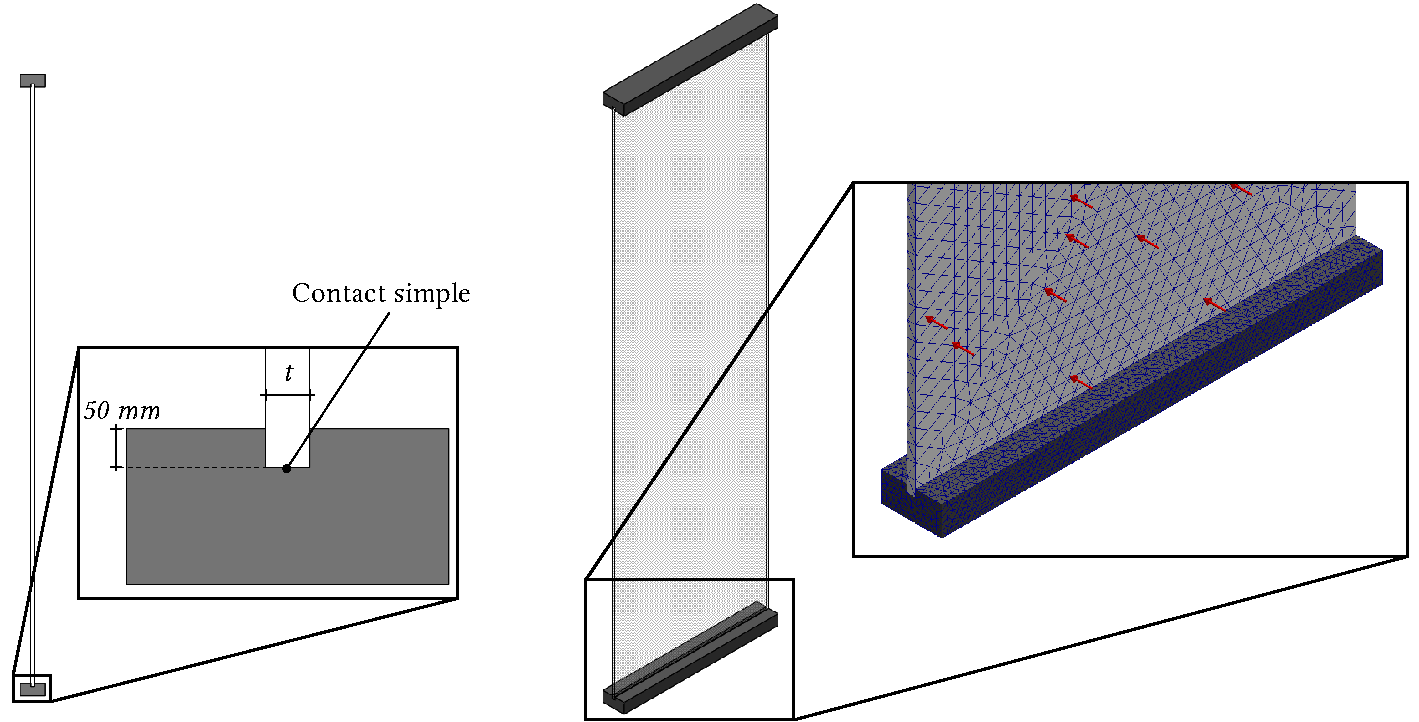
\includegraphics[width=\textwidth]{img/plat/fem.pdf}
    \caption{Géométrie et maillage SOLIDWORKS du verre plat.}
    \label{fig:fem_plat}
\end{figure}

On applique à un des deux côtés du verre une pression uniforme (à l'\acrshort{ELU}: \qty{3}{\kilo\pascal}) et on soumet l'ensemble à une gravité (à l'\acrshort{ELU}: \qty{13.5}{\metre\per\squared\second}). Les caractéristiques matériaux utilisés dans ce calcul et dans tous les suivants sont répertoriés dans le tableau \ref{tab:mat_autoportant}. 

On effectue finalement une analyse linéaire donnant la contrainte, selon le critère Von Mises, dans le verre. 

\begin{table}[H]
\begin{center}
\caption{Description des matériaux utilisés dans les \acrshort{FEM}.}
\label{tab:mat_autoportant}
\begin{tabularx}{\textwidth}{l*{5}{Y}}
\toprule
\textbf{Matériau} & \textbf{Module d'Young} $E$ [MPa] & \textbf{Module de cisaillement} $G$ [MPa]&\textbf{Coefficient de poisson} $\nu$ & \textbf{Limite d'élasticité} $f_y$ [MPa]& \textbf{Masse volumique} $\rho$ [kg/m$^3$] \\\midrule
Verre durci & 72$\times 10^3$ & 29.5$\times 10^3$ & 0.22 &45 & 2457 \\
Verre trempé & 72$\times 10^3$ & 29.5$\times 10^3$ & 0.22 &70 & 2457 \\
DOWSIL™ 895 & 1.0 & 0.33 & 0.499 & 1.06* & 1430 \\
DOWSIL™ 781 & 0.4 & 0.13 & 0.499 & 1.8* & 1020 \\
Silicone & 4.5 & 1.5 & 0.499 & 4.5* & 1000\\
\bottomrule
\end{tabularx}
\end{center}
{\RaggedLeft \footnotesize * Valeur de limite d'élasticité prise égale à la limite en traction.}\end{table}

Cette méthodologie de calcul \acrshort{FEM} sera utilisée dans toute la suite du mémoire.

\begin{figure}[H]
    \centering
    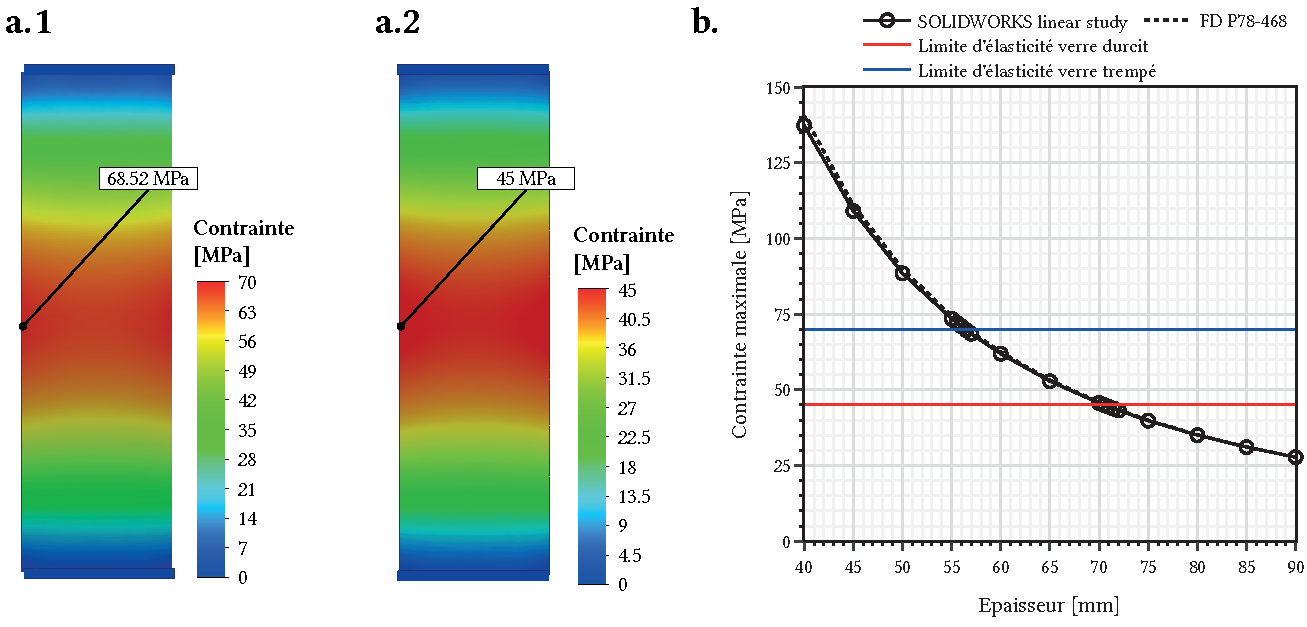
\includegraphics[width=\textwidth]{img/plat/dim_fem.pdf}
    \caption{Résultats du calcul \acrshort{FEM} du verre plat. \textbf{a.} Profil des contraintes dans le verre (\textbf{1.} verre trempé, \qty{56.5}{\milli\meter} et \textbf{1.} verre durci, \qty{70.5}{\milli\meter}) et \textbf{b.} contrainte maximale dans le verre en fonction de son épaisseur pour le verre trempé et le verre durci.}
    \label{fig:fem_plat_dim}
\end{figure}

En traçant la contrainte maximale calculée par \acrshort{FEM} dans le verre en fonction de son épaisseur on observe des résultats très proche du calcul du document \Textcite{fdp78}, c'est-à-dire du calcul analytique d'une poutre sur deux appuis. On trouve ainsi une épaisseur minimale légérement inférieure à celle calculée précédemment: \qty{70.5}{\milli\meter} pour le verre trempé et \qty{56.5}{\milli\meter} pour le verre durci. Un rapide calcul \acrshort{FEM} au flambement nous donne des coefficients de flambement respectifs de 10.887 et 16.943: il n'y a pas de risque de flambement avec ces épaisseurs de verre. 
\newpage

\section{Optimisation géométrique du verre}

Introduction sur l'optimisation géométrique... Gain en inertie, section en I pour l'acier etc...
blablabla courber le verre pour l'architecture, mettre photo d'architectures avec verre courbe (zaha hadid)
mais on peut le courber pour que ça soit intéressant structurellement.

\newpage
\subsection{Le verre ondulé}

En s'inspirant de l'historique des tôles d'acier ondulées nous pouvons explorer le potentiel du verre ondulé. En effet, l'ondulation des tôles d'acier a permis d'augmenter considérablement la rigidité des éléments surfaciques d'acier tout en réduisant leur épaisseur et leur poids. Les tôles ondulées sont d'ailleurs ajourd'hui largement utilisées dans la construction, que ça soit en guise de couverture, de façade ou bien en collaboration avec du béton pour la réalisation de planchers.

On peut retrouver le verre ondulé dans certains projets construits, principalement en raison de son attrait esthétique. Contrairement aux tôles d’acier, souvent associées à une architecture plutôt industrielle, l’ondulation du verre permet de créer des effets visuels innovants, jouant sur les reflets, la transparence, et la diffraction de la lumière, comme on peut l'observer dans des projets tels que la Casa Da Mùsica de Porto ou la Qatar National Library. 

\begin{figure}[H]
    \centering
    \includegraphics[height=0.392\textwidth]{img/ondul/casa_musica4 (1).jpg}\hfill
    \includegraphics[height=0.392\textwidth]{img/ondul/casa_musica1 (1).jpg}
    \\[\smallskipamount]
    \includegraphics[height=0.331\textwidth]{img/ondul/02_Qatar_National_Library__Photo_by_Hans_Werlemann_4180.jpg}\hfill
    \includegraphics[height=0.331\textwidth]{img/ondul/07_Qatar_National_Library__Photo_by_Iwan_Baan_5345.jpg}
    \caption{Photographies de la façade en verre ondulé de la Casa Da Música de Porto, par \Textcite{CasaDaMusica} (première ligne) et de la Qatar National Library, par \Textcite{quatNatLib} et \Textcite{quatNatLib2} (seconde ligne).}
    \label{fig:CasaDaMusica}
\end{figure}

Dans cette partie nous allons donc étudier le bénéfice possible d'un vitrage autoportant en verre ondulé. Nous traiterons tout d'abord les formes d'ondulations possibles, puis nous étudierons le comportement d'un verre autoportant ondulé et nous finirons par un dimensionnement.

\subsubsection{Forme des ondulations}
On peut s'intéresser à deux formes d'ondulation que l'on retrouve dans les tôles d'aciers ondulés ou dans les façades en verre ondulé: les ondulations sinusoïdale et circulaire. 

La première est simplement obtenue en prenant une onde sinusoïdale de longueur d'onde correspondant à la largeur du vitrage et d'amplitude fixées. La seconde est constituée de deux arcs de cercles issus de cercles tangents.

\begin{figure}[H]
    \centering
    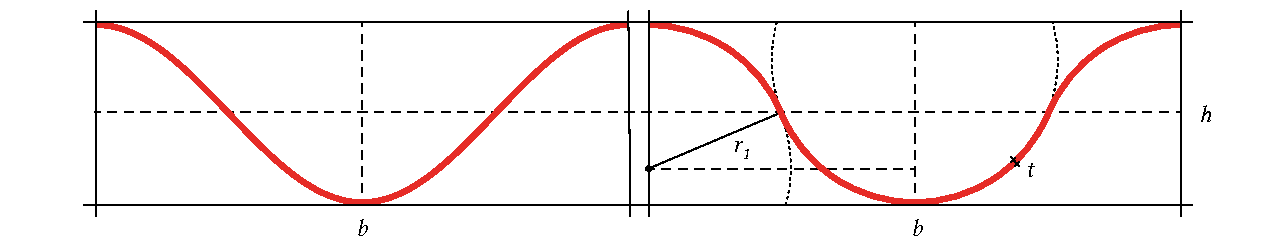
\includegraphics[width=\linewidth]{img/ondul/circ.pdf}
    \caption{Schéma d'une longueur d'onde sinusoïdale \textit{(à gauche)} et circulaire \textit{(à droite)}.}
    \label{fig:ondcirc}
\end{figure}

L'ondulation sinusoïdale ne dépend que de deux paramètres: sa longueur d'onde $b$ et sa hauteur (son amplitude) $h$. Ainsi sa section et son inertie ne dépend que de $b$, $h$ et $t$.

Ce n'est pas le cas de l'ondulation circulaire qui dépend en plus d'un rayon $r_1$, le rayon du premier arc de cercle de l'onde comme noté sur la figure \ref{fig:ondcirc}. En posant le paramètre $\theta = 2 \tan^{-1} \frac{b-2h}{b+2h}$, on peut remarquer que sa section est égale à:
\begin{align}
    S_{\text{circ}} = \frac{b^2+4h^2}{8h} \left ( \frac{\pi}{2} - \theta\right )t
\end{align}
Ainsi la section de l'ondulation circulaire ne dépend, tout comme l'ondulation sinusoïdale, que de $b$, $h$ et $t$. En d'autres termes, faire varier la paramètre $r_1$ changera l'inertie de la section mais pas la quantité de verre utilisée pour mettre en oeuvre un tel vitrage.  Il est donc intéressant de chercher la rayon donnant la plus grande inertie à $b$, $h$ et $t$ fixés.

\begin{figure}[H]
    \centering
    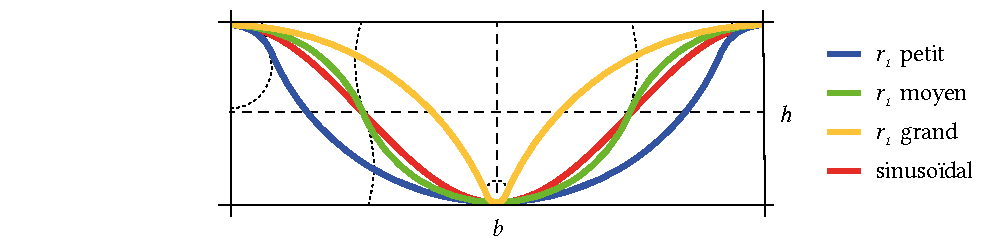
\includegraphics[width=0.8\linewidth]{img/ondul/circ2.pdf}
    \caption{Schéma comparant les ondulations circulaires pour différents rayons $r_1$.}
    \label{fig:ondcirc2}
\end{figure}
L'ondulation circulaire est formée de deux arcs de cercles de telle sorte que la somme soit de leur rayon soit constante à $h$ et $b$ fixés. Intuitivement, augmenter ou faire diminuer $r_1$ augmentera le rayon de courbure de l'ondulation (puisque si $r_1$ diminue, le rayon du cercle central augmente), ce qui aura pour effet de diminuer l'inertie de la section. Ainsi, l'ondulation idéale serait lorsque les deux rayons sont égaux, ce qui peut-être démontré par le calcul mais nous ne le ferons pas ici. Dans ce cas, 
\begin{align}
    r_1 = \frac{b^2+4h^2}{16h}
\end{align}

\begin{figure}[H]
    \centering
    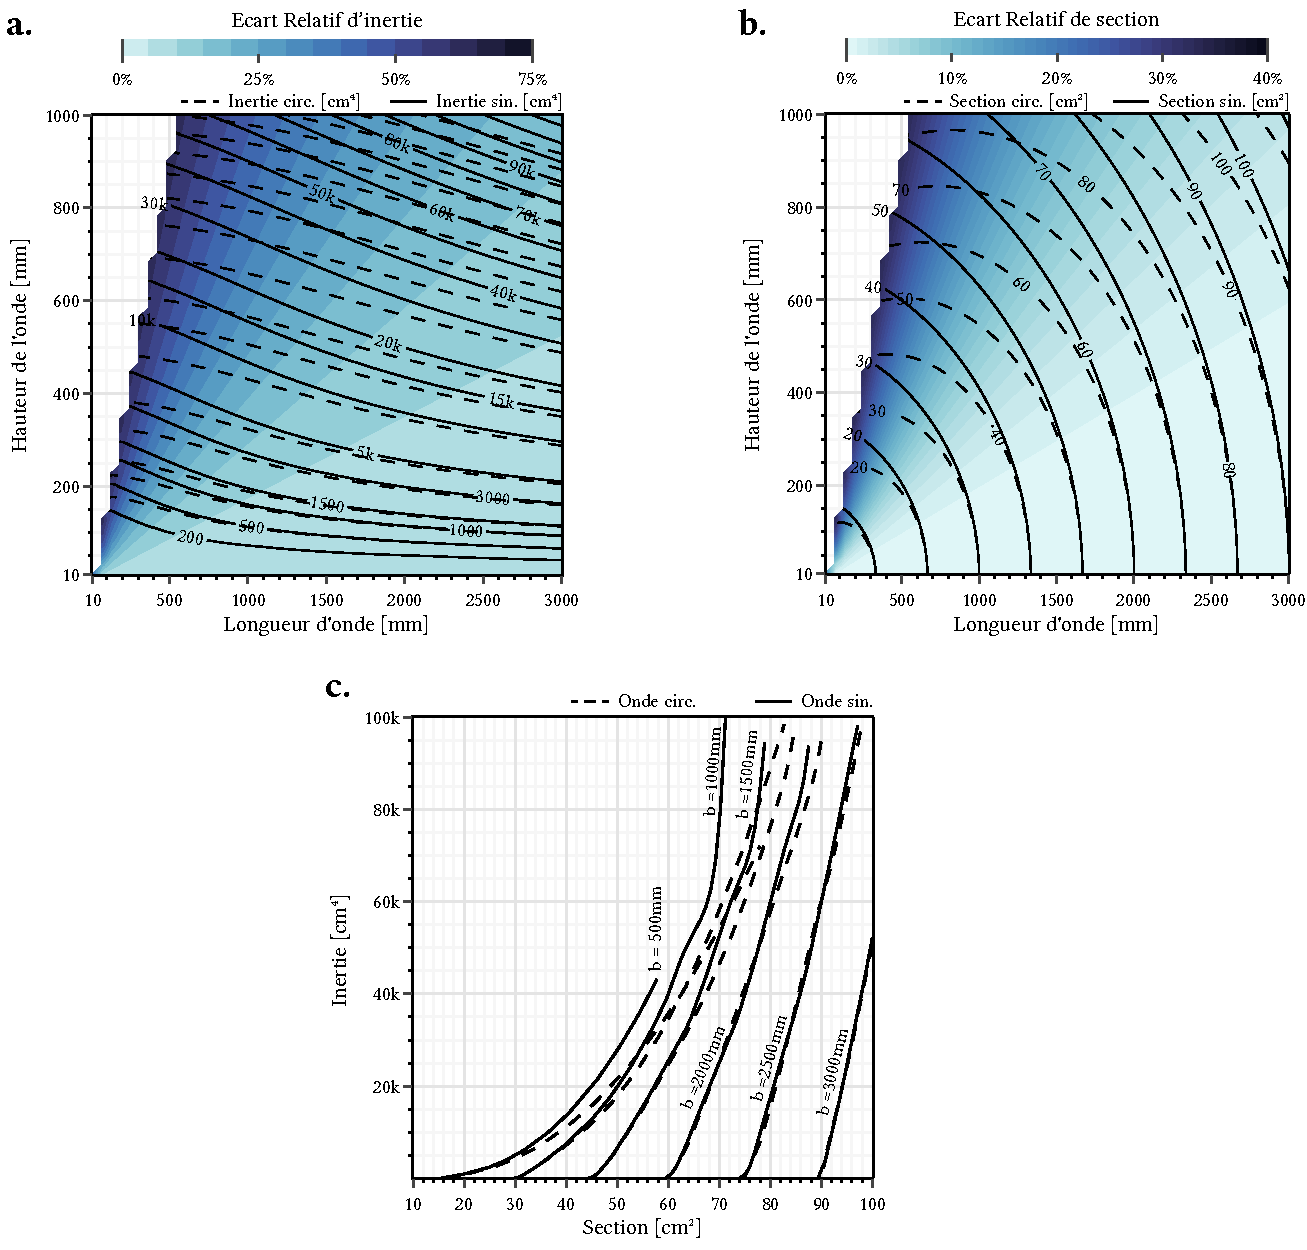
\includegraphics[width=\linewidth]{img/ondul/section_circ.pdf}
    \caption{\textbf{a.} et \textbf{b.} Écart relatif entre l'inertie et la section respectivement, de l'onde sinusoïdale et de l'onde circulaire optimale selon la longueur d'onde et la hauteur de l'onde. \textbf{c.} Inertie de l'onde selon sa section pour différentes longueur d'onde.}
    \label{fig:ERcirc}
\end{figure}
C'est le cas de l'ondulation verte schématisée sur la figure \ref{fig:ondcirc2}. Cette ondulation se rapproche de celle sinusoïdale. On peut d'ailleurs comparer l'écart relatif, $ER = \frac{I_{\text{circ}}-I_{\text{sin}}}{I_{\text{sin}}}\times 100\%$, entre les inerties de l'ondulation sinusoïdale et de l'optimum circulaire en fonction de la longueur d'onde $b$ et la hauteur de l'onde $h$. Cet écart relatif est mis en parallèle de l'écart relatif sur la section dans le figure \ref{fig:ERcirc}.
\\

Les écarts relatifs entre l'ondulation sinusoïdale et circulaire sont croissants en $\frac{h}{b}$. Comme la figure \ref{fig:ondcirc2} pouvait le laisser penser, à $b$ et $h$ fixés, l'inertie et la section de l'onde circulaire sont toujours supérieurs à celles de l'onde sinusoïdale. 
\\

Il est intéressant de regarder, pour une même quantité de verre, quelle onde sera la plus intéressante structurellement. En d'autres termes, pour une même section et une même longueur d'onde, quelle onde aura la meilleure inertie. Lorsque l'on fixe ces deux paramètres, on obtient une hauteur d'onde différente pour l'onde circulaire est sinusoïdale, comme présenté dans le graphique \textbf{b.} de la figure \ref{fig:ERcirc}. L'écart entre ces deux hauteurs d'ondes est d'autant plus grande que la section $S$ est grande.

  Cependant, cette différence de hauteur d'onde n'implique pas une aussi grande différence d'inertie. Ainsi, on obtient que pour des grandes valeurs de section, l'inertie de la section circulaire est plus petite que celle de la section sinusoïdale: il est nécessaire d'aplatir l'onde circulaire pour conserver la même section. Le graphique \textbf{c.} confirme ce résultat et montre également que la différence d'inertie est d'autant plus grande que $b$ est petit.

  Le choix de la forme d'ondulation est un compromis à faire entre la volonté architecturale et l'économie de matériau. Pour une même quantité de matériau, l'amplitude de l'ondulation peut-être jusqu'à 25\% plus petite pour l'onde circulaire par rapport à l'onde sinusoïdale. Toutefois, à  section et longueur d'onde égale, l'ondulation sinusoïdale a très souvent une meilleure inertie.
  \\
  
Dans la suite nous nous concentrerons sur l'ondulation sinusoïdale.
\subsubsection{Autoportance}
En plus de l'avantage inertiel du verre ondulé par rapport au vert plat, il profite également d'une meilleure stabilité de part son amplitude d'oscillation. Il peut donc être intéressant de l'utiliser de façon autoportant sans prise en feuillure latérale. 

On étudie, dans la suite, le verre ondulé autoportant soumis à une charge de vent et à son poids propre. On prendra notamment une charge de vent égale à $\text{W} = \qty{1000}{\pascal}$ et on considérera un vitrage formé de 3 ondulations sinusoïdales.


\paragraph{Première approche analytique linéaire}\mbox{}

En première approximation on peut modéliser la situation par une poutre de longueur $L$, isostatique sur deux appuis simples, de section $S_{\text{sin}}$ et d'inertie $I_{\text{sin}}$, la section et l'inertie de son ondulation.



Le poids propre du vitrage est simplement pris égal à: 
\begin{align}
    g = \frac{\rho_{\text{verre}}}{100} S_{\text{sin}} \text{ }\unit{\kilo\newton/\meter}
\end{align}
tandis que la charge surfacique de vent doit être convertie en charge linéique le long de la hauteur du vitrage. Ce qui nous intéresse, pour notre première approximation, est la résultante du vent dans le sens de la hauteur du profil, i.e. sans prise en compte de la résultante s'appliquant latéralement sur la section.
\begin{wrapfigure}{l}{0.3\textwidth}
    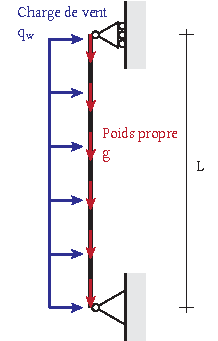
\includegraphics[width=\linewidth]{img/ondul/schem_stat.pdf}
       \caption{Schéma statique du verre ondulé dans une première approximation.}
   \label{fig:ondul_stat}
   \end{wrapfigure}
Pour cela on présente, dans la figure \ref{fig:ondul_cas}, deux approches. La première est simple: on suppose que le vent agit comme une charge de neige indépendamment de la forme du profil. Sa résultante dans le sens de la hauteur du profil (selon $\underline{e_y}$) est alors:
\begin{align}
    \sum f_y = -q\times b 
\end{align}

Le second cas est le cas réel: le vent s'applique perpendiculairement à la surface en tout point du profil. Dans ce cas, comme précisé dans la figure \ref{fig:ondul_cas}, on peut étudier un bout de section infinitésimal entre $x$ et $x+\mathrm{d}x$. La longueur de cet élément est $\mathrm{d}l = \frac{\mathrm{d}x}{\cos \alpha}$. La force appliquée à l'élément s'écrit:
\begin{align}
    \underline{\mathrm{d}f} = \mathrm{d}l q \left (\sin \alpha \underline{e_x} - \cos \alpha \underline{e_y}\right )
\end{align}
Donc sa résultante selon $\underline{e_y}$ est simplement donnée par:
\begin{align}
    \mathrm{d}f_y = - \mathrm{d}l q\cos \alpha = -q \times \mathrm{d}x
\end{align}
\\[0.5cm]

\begin{wrapfigure}{r}{0.5\textwidth}
    \vspace{-30pt}
    \centering
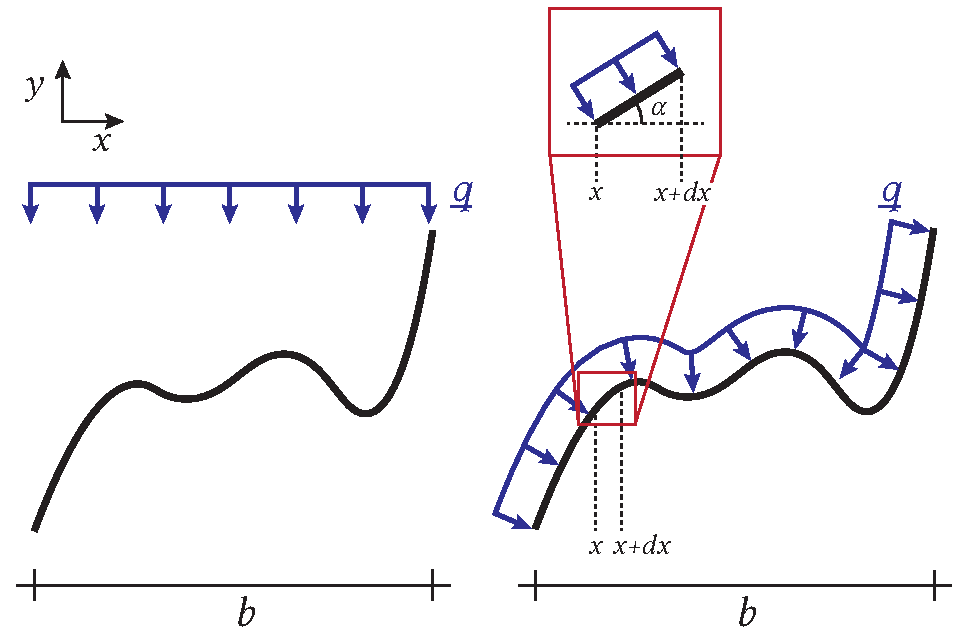
\includegraphics[width=0.9\linewidth]{img/ondul/proj_load.pdf}
\caption{Schémas de l'application de la charge de vent sur la section du verre ondulé.}
\label{fig:ondul_cas}
\vspace{10pt}
\end{wrapfigure}

Ainsi, la résultante totale sur toute la section est:
\begin{align}
    \sum f_y = \int \mathrm{d}f_y = \int_0^b -q \mathrm{d}x = -q\times b \label{eq:fy}
\end{align}


On en déduit qu'en terme de résultante selon $\underline{e_y}$, les deux cas sont équivalents.

A noté que si l'on revient au cas d'une section sinusoïdale, la symétrie du profil implique que la résultante selon $\underline{e_x}$ de la charge est nulle. 

On prend donc, dans notre première approximation, une charge linéique de vent s'appliquant à la poutre égale à:

\begin{align}
    q_{\text{w}} = \text{W} \times b
\end{align}
On en déduit la contrainte maximale dans le verre: 
\begin{align}
    \sigma_{\text{max}} = \frac{\num{3d-3} b L^2}{16 I_{\text{sin}}}h + \num{1.228d-2} L\text{ }\unit{\mega\pascal}
\end{align}
et le déplacement:
\begin{align}
    U_y = \frac{\num{15d-3} b L^4}{384 E_{\text{v}}I_{\text{sin}}}
\end{align}

\paragraph{Prise en compte de la torsion dans la section}\mbox{}

Pour aller un peu plus loin, on peut prendre en compte la composante dans la direction longitudinale du profil (i.e. selon $\underline{e_x}$ d'après la figure \ref{fig:ondul_cas}). 

\begin{wrapfigure}{l}{0.35\textwidth}
\centering
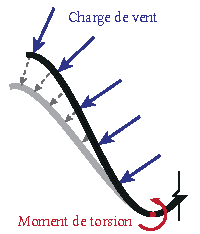
\includegraphics[width=0.8\linewidth]{img/ondul/torsion.pdf}
\caption{Schéma de la torsion engendrée par l'effet du vent dans la section.}
\label{fig:tors_ondul}
\vspace{10pt}
\end{wrapfigure}

Cette composante engendre des contraintes supplémentaires dus à la torsion de la section, comme schématisé dans la figure \ref{fig:tors_ondul}.

Par un calcul semblable à celui réalisé précédemment, on montre que le moment engendré par la composante selon $\underline{e_x}$ du vent est égal au moment créé au pied d'une console de longueur $h$:
\begin{align}
    M_{\text{tors}} = \frac{q h^2}{2}
\end{align}

Ainsi la contrainte supplémentaire dans le verre est:
\begin{align}
    \sigma_{\text{tors}} = \frac{3\text{W}\times h^2}{t^2} = \num{3d-3} \frac{h^2}{t^2}\text{ }\unit{\mega\pascal}
\end{align}

Ce qui nous donne la nouvelle contrainte maximale:
\begin{align}
    \sigma_{\text{max}} = \frac{\num{3d-3} b L^2}{16 I_{\text{sin}}}h + \num{1.228d-2} L + \num{3d-3} \frac{h^2}{t^2}\text{ }\unit{\mega\pascal}\label{eq:s_maxondul}
\end{align}
\paragraph{Calcul \acrshort{FEM}}\mbox{}

Pour comparer nos résultats analytiques, on effectue un calcul statique linéaire \acrshort{FEM} à l'aide du logiciel SOLIDWORKS. On considère un vitrage de 3m de haut et formé de 3 ondes de 300mm de longueur d'onde et de 3mm d'épaisseur. On modélise la prise en feuillure sur les bords hauts et bas du vitrage par une un contact simple avec deux parallélépipèdes en silicone dans lesquels le vitrage est inséré sur 15mm à l'instar des vitrages dans la Casa Da Música de Porto. Le verre est libre de se déplacer autrement. Les propriétés des matériaux utilisés dans l'analyse sont décrites dans le tableau \ref{tab:mat_autoportant}.

La géométrie des éléments et le maillage est présenté dans la figure \ref{fig:ondulmaill}. Les parallélépipèdes en silicone sont fixés sur 5 de leurs côtés. La charge surfacique de vent est prise perpendiculaire à la surface du verre.

\begin{figure}[H]
    \centering
    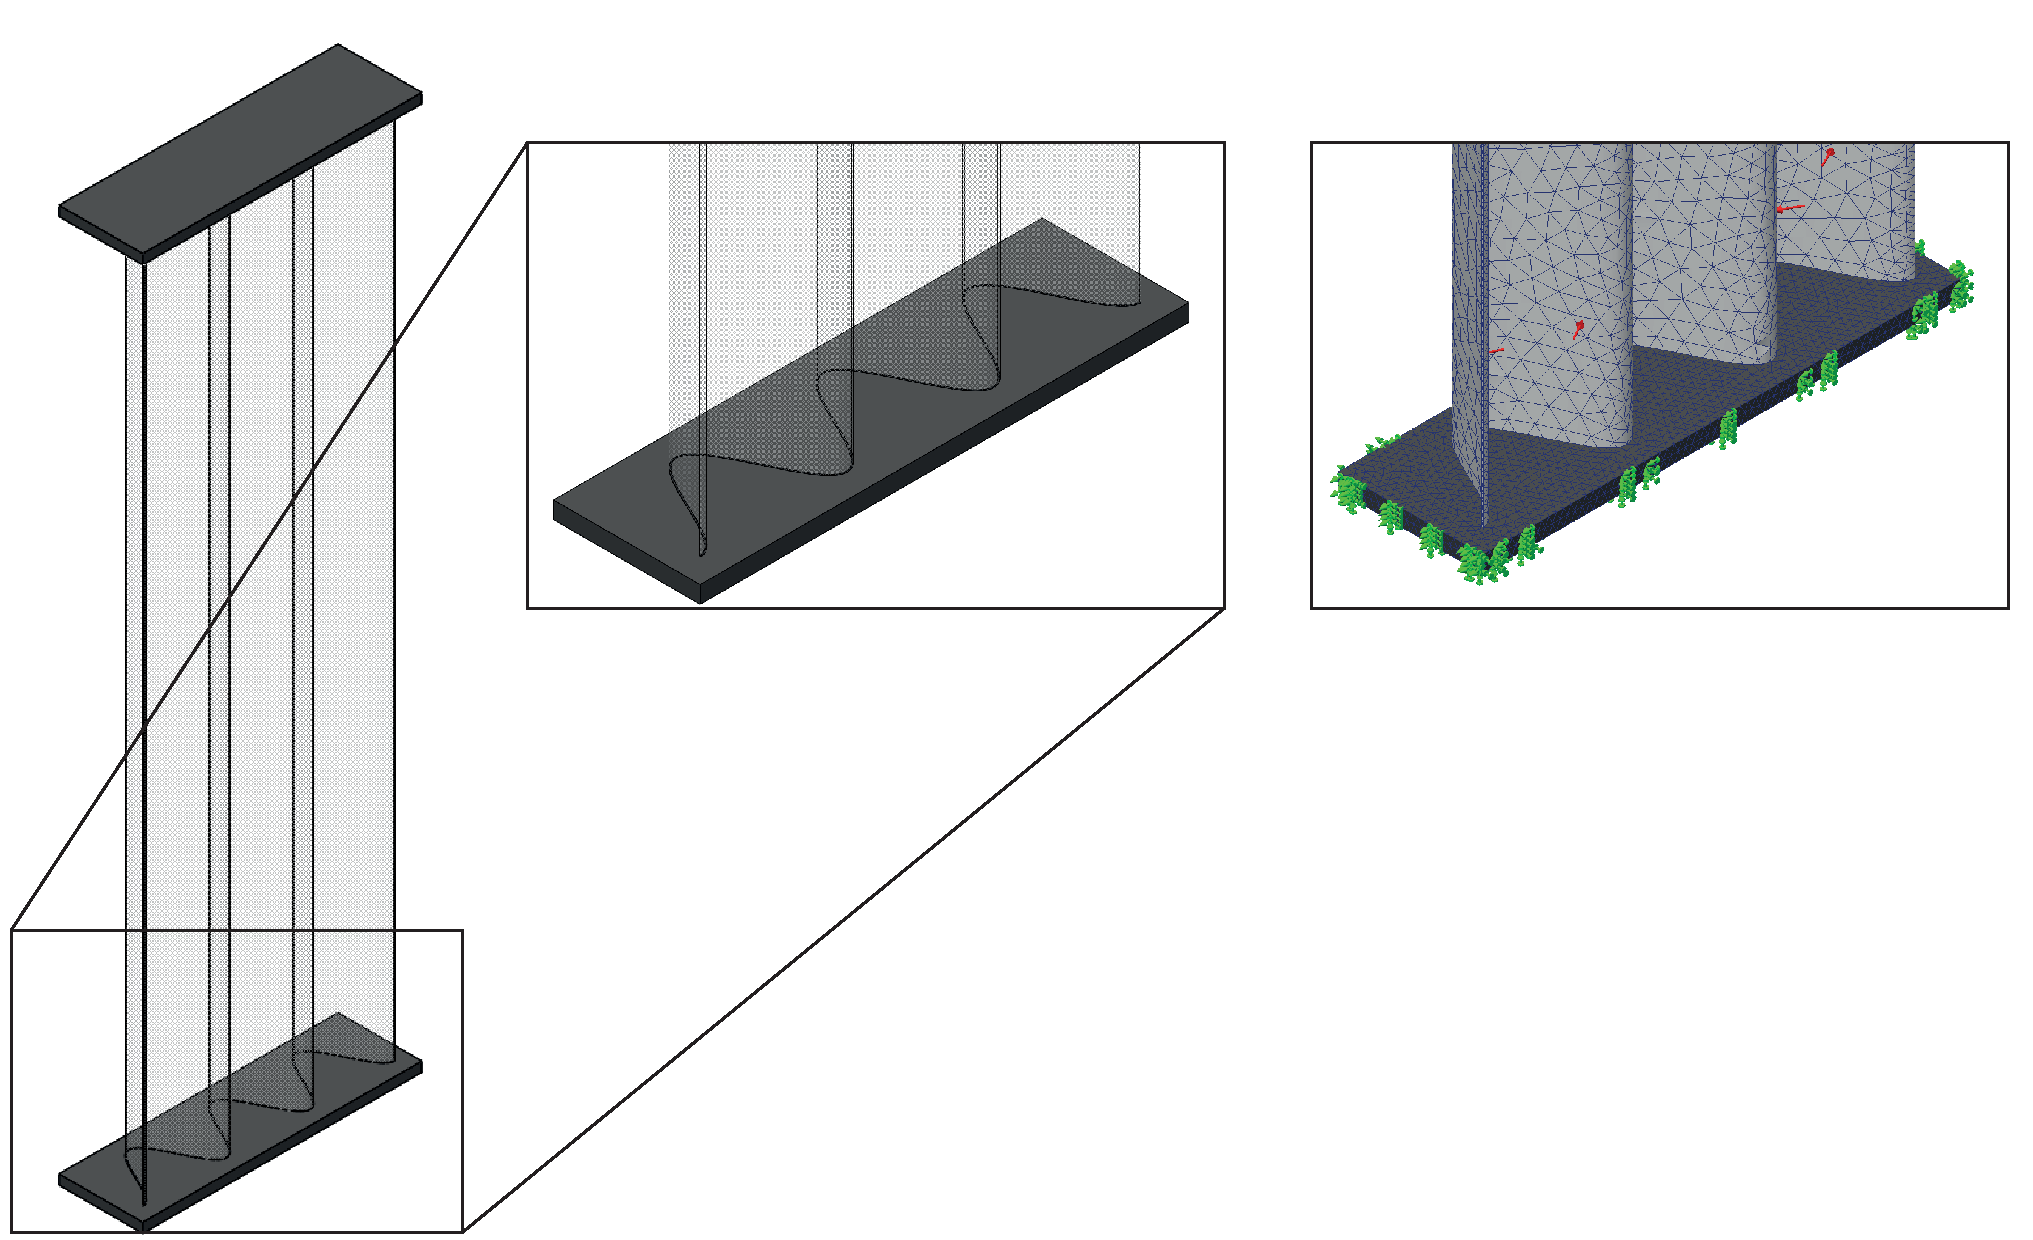
\includegraphics[width=0.8\linewidth]{img/ondul/fem/maillage_simple.pdf}
    \caption{Géométrie et maillage SOLIDWORKS du verre ondulé simple.}
    \label{fig:ondulmaill}
\end{figure}

On peut comparer les résultats obtenus par \acrshort{FEM} pour trois amplitudes d'ondulation, \qty{10}{\milli\meter} et \qty{200}{\milli\meter}, présentés dans la figure \ref{fig:ondulfemscreen}. 

Les contraintes maximales se situent au niveau des crêtes dans les creux du vent bien qu'on puisse trouver de très fortes contraintes ponctuellement au niveau de la jonction avec le silicone ce qui n'est dû qu'aux contraintes de notre modélisation. L'emplacement de ces contraintes maximales sont en accord avec nos intuitions sur la torsion présente dans la section du verre discutée précédemment. De plus, la contrainte maximale calculée pour une amplitude d'onde de \qty{100}{\milli\meter} est plus faible que pour les amplitudes \qty{10}{\milli\meter} et \qty{200}{\milli\meter}. On pouvait intuiter ce résultat avec l'équation (\ref{eq:s_maxondul}). La contrainte engendrée par le moment de flexion est en $\frac{h}{I_{\text{sin}}}$ ce qui, comme $I_{\text{sin}}$ est plus que linéaire en $h$ d'après la figure \ref{fig:ERcirc}, décroît lorsque $h$ augmente. A contrario, la contrainte engendrée par la torsion de la section croît en $h^2$. Il y a donc une bataille entre ces deux termes: si $h$ est trop grand, la torsion sera importante tandis que si $h$ est trop petit, l'ondulation aura peu d'impact sur l'inertie.

\begin{figure}[H]
    \centering
    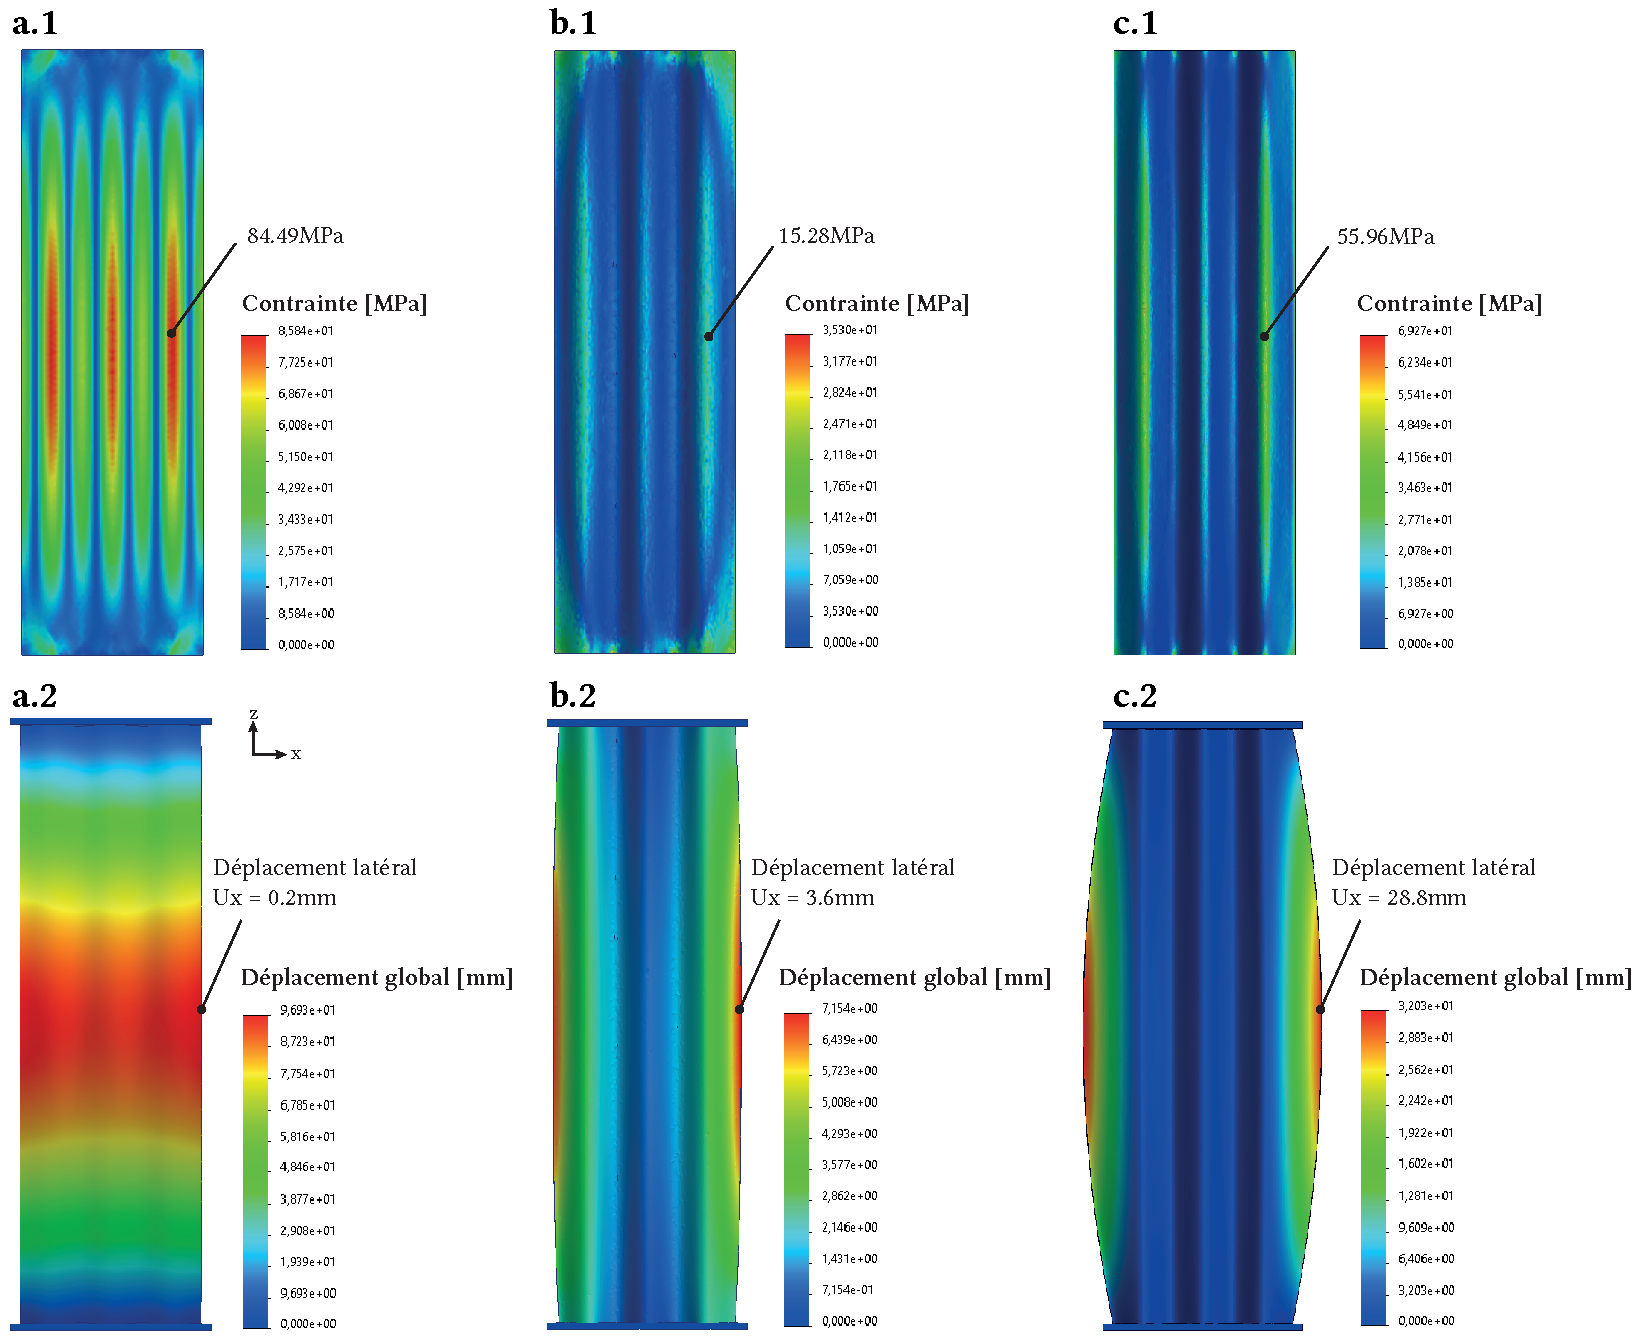
\includegraphics[width=\linewidth]{img/ondul/fem/FEM1.pdf}
    \caption{\textbf{1.} Contrainte et \textbf{2.} déplacement global ($U = \sqrt{U_x^2 + U_y^2 + U_z^2}$, échelle x5) du verre ondulé pour trois différentes amplitudes d'ondulation: \textbf{a.} 10mm, \textbf{b.} 100mm et \textbf{c.} 200mm. Les échelles de couleur sont toutes différentes.}
    \label{fig:ondulfemscreen}
\end{figure}

On observe également un déplacement latéral important au niveau des bords du vitrage. Ce déplacement est d'ailleurs à prendre en compte afin de réaliser une façade en verre ondulé: le verre ne doit pas trop se déplacer latéralement pour éviter le contact avec les autres verres.

Les résultats \acrshort{FEM} et analytiques pour plusieurs hauteurs d'ondulation entre \qty{10}{\milli\meter} et \qty{300}{\milli\meter} sont présentées dans la figure \ref{fig:ondulfem1}. 

Les résultats obtenus numériquement diffèrent de la première approximation analytique. La contrainte est d'abord une fonction décroissante de $h$ jusqu'à atteindre un minimum autour de \qty{75}{\milli\meter}, puis croissante. Cela confirme notre intuition sur la tension engendrée par la forme de la section puisque, pour la contrainte maximale dans la crête centrale, l'allure de la contrainte semble clairement être proche de la courbe donnée par l'équation (\ref{eq:s_maxondul}). Toutefois, pour les crêtes latérales, la contrainte diverge beaucoup plus rapidement, ce qui peut-être expliqué par la non symétrie en ce point, contrairement à la crête centrale. 

Le résultat analytique simple sur-évalue les contraintes et le déplacement transversal du verre, notamment de par la modélisation du problème en poutre et non en plaque. 

\begin{figure}[H]
    \centering
    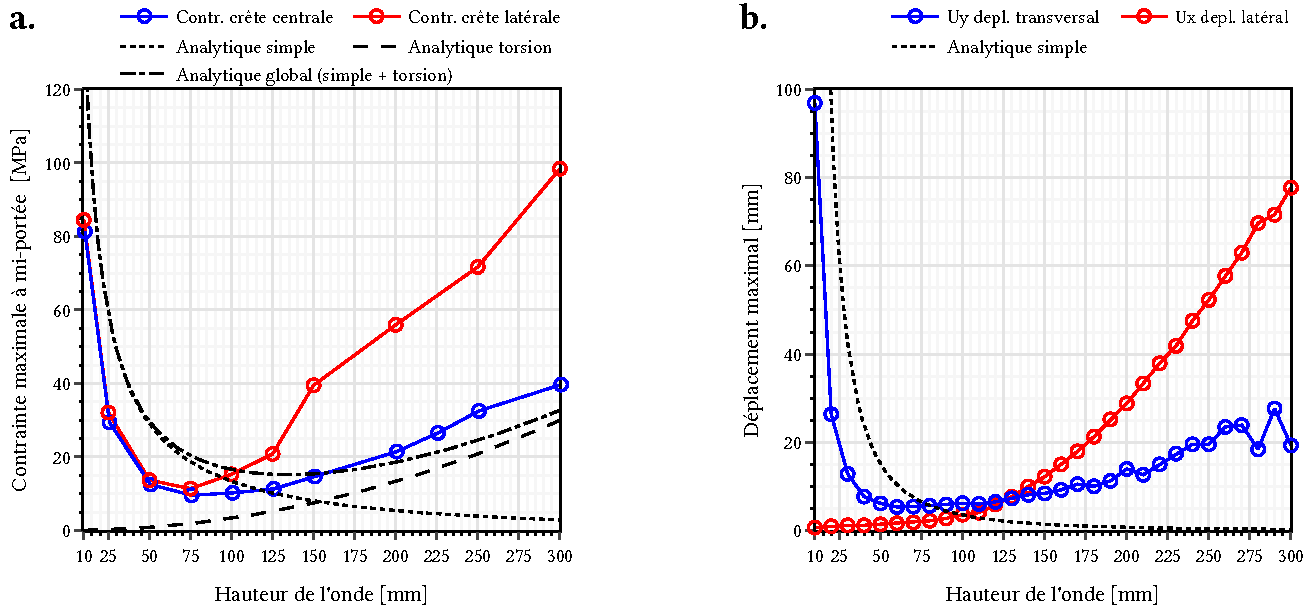
\includegraphics[width=\linewidth]{img/ondul/fem/simple_fem.pdf}
    \caption{\textbf{a.} Contrainte maximale à mi-portée et \textbf{b.} déplacement maximal du verre ondulé selon l'amplitude de l'onde par un calcul analytique et un calcul \acrshort{FEM}.}
    \label{fig:ondulfem1}
\end{figure}



Ainsi, notre modèle tenant compte de la torsion, donné par l'équation (\ref{eq:s_maxondul}), permet de donner une bonne approximation de la contrainte dans le crête centrale, bien qu'elle sur-évalue les contraintes pour les plus petites hauteurs d'onde. Un meilleure modèle pour évaluer les contraintes dus à la flexion permettraient de se rapprocher du résultat \acrshort{FEM}. Bien qu'il ne permette pas de rendre compte des contraintes dans les crêtes latérales, un tel modèle est suffisant pour calculer un verre ondulé avec beaucoup d'ondes dont on maintiendrait les bords.


\subsubsection{Collaboration entre les vitrages}

En réalité il est difficile de produire des verres de très grandes largeurs et il est nécessaire d'accoler plusieurs vitrages. Pour des raisons de simplicité de production et d'installation, un panneau de verre ne sera composé que d'une seule onde, comme c'est le cas pour la façade de la Casa Da Música de Porto ou de La Samaritaine à Paris.

Il est nécessaire, entre deux panneaux de verre autoportants côte à côte sur une façade, d'ajouter un morceau de silicone, ponctuellement ou de façon linéaire sur tout le bord, afin d'éviter le contact entre les deux verres. Plusieurs cas sont possibles pour le positionnement du joint en fonction de la découpe de l'onde. La séparation entre les panneaux de verre peut se faire au niveau de l'axe neutre de l'onde, comme c'est le cas de la façade de La Samaritaine à Paris, ou bien au niveau des crêtes, comme pour la façade de la Casa Da Música de Porto. On choisit d'étudier ces deux cas pour le joint. On effectue donc un calcul \acrshort{FEM}, comme présenté dans la figure \ref{fig:jointsq}, pour les deux situations évoqués ainsi que pour un verre sans joint, à titre de comparaison. Les matériaux utilisés sont les mêmes que ceux décrits dans la table \ref{tab:mat_autoportant}. La longueur d'onde du verre est prise égale à \qty{300}{\milli\metre} et sa hauteur à \qty{75}{\milli\metre}. Les joints remplissent tout l'espace entre les verres. Cette distance est prise égale à \qty{5}{\milli\meter}. Les joints sont donc des parallélépipèdes de dimension \qtyproduct{3 x 5 x 3000}{\milli\metre}. Afin de pouvoir approcher le comportement d'une façade comportant plusieurs panneaux de verres autoportants on effectue le calcul \acrshort{FEM} avec 7 pièces de verre ondulé et on s'intéresse uniquement au comportement du verre central. Les bords latéraux des ensembles de verres sont contraints de sorte à ne pas bouger latéralement.

\begin{figure}[H]
    \centering
    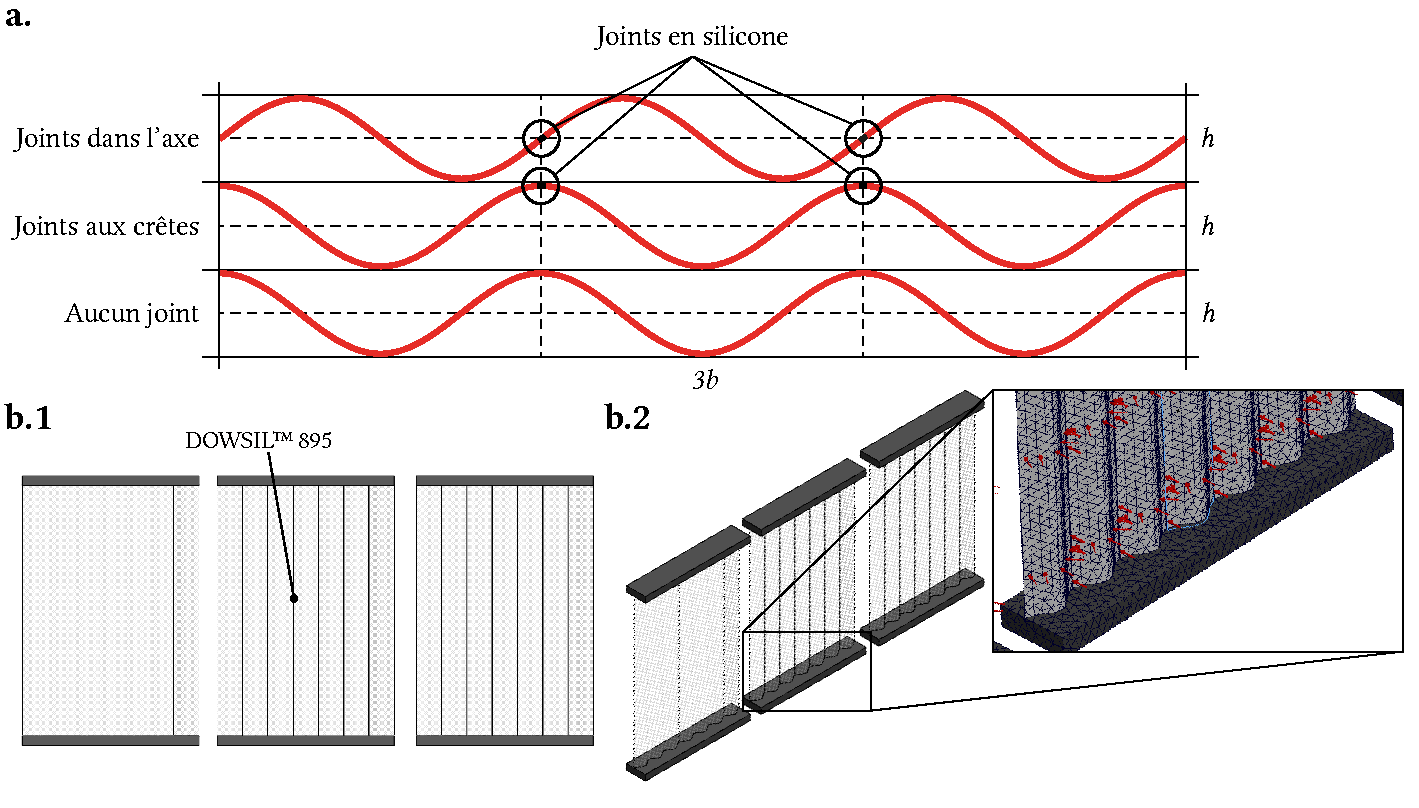
\includegraphics[width=\linewidth]{img/ondul/jointsq.pdf}
    \caption{\textbf{a. }Schéma des différents cas de jointure entre les verres ondulés étudiés. \textbf{b.} Modèles \acrshort{FEM} des trois différents cas de jointure (\textbf{1.} élévation; \textbf{2.} axonométrie).}
    \label{fig:jointsq}
\end{figure}

Les résultats sont présentés dans le figure \ref{fig:femjoints}. On peut, en premier lieu, observer l'allure de la déformée du verre. La déformée est semblable pour le verre sans joint et celui avec joints aux crêtes. Ce déplacement est principalement transversal (i.e. perpendiculairement au plan du vitrage). En revanche, le déplacement latéral n'est pas négligeable pour le verre avec des joints dans l'axe. Cela s'explique par le dissymétrie du profil par rapport à l'effet du vent. La partie du profil ouverte face au vent va se déplier tandis que la partie fermée va se replier. Ainsi mettre des joints dans l'axe de l'ondulation va engendrer une plus grande instabilité du verre de part l'ajout du silicone qui est bien moins rigide. Ce résultat est confirmé par le profil des contraintes dans le verre. Les contraintes dans le verre avec les joints dans l'axe sont bien plus importantes que dans les autres cas.

En effet, relativement au cas sans joint, la contrainte maximale dans le cas des joints aux crêtes n'augmente pas tandis que pour les joints dans l'axe, elle augmente de 66\%.  

\begin{figure}[H]
    \centering
    \includegraphics[width=\linewidth]{img/ondul/fem/femjoint.pdf}
    \caption{\textbf{a.} Résultats du calcul \acrshort{FEM} pour les trois cas de joints: sans joints, aux crêtes et dans l'axe (\textbf{1.}: vent en pression et \textbf{2.} vent en dépression).}
    \label{fig:femjoints}
\end{figure} 


L'ajout des joints dans l'axe semble avoir un effet sur les contraintes par rapport à un verre sans aucun joints. En effet, on observe une augmentation des contraintes en pied et en tête du verre mais une diminution au niveau des joints. Cela s'explique par la faible rigidité du joint en silicone qui va permettre au verre de plus se déformer. Or, en pied et en tête, sous l'effet de la pression du vent, le verre ondulé de par sa forme, va se rétracter latéralement. Cette rétractation va engendrer de la flexion au niveau du creux et donc une augmentation des contraintes dans cette zone. Tandis qu'a mi-portée, le verre s'étend, donnant lieu à de la compression dans le joint qui, plus souple que le verre, va permettre une diminution des contraintes. 
\newpage
\begin{wrapfigure}{l}{0.5\textwidth}
\centering
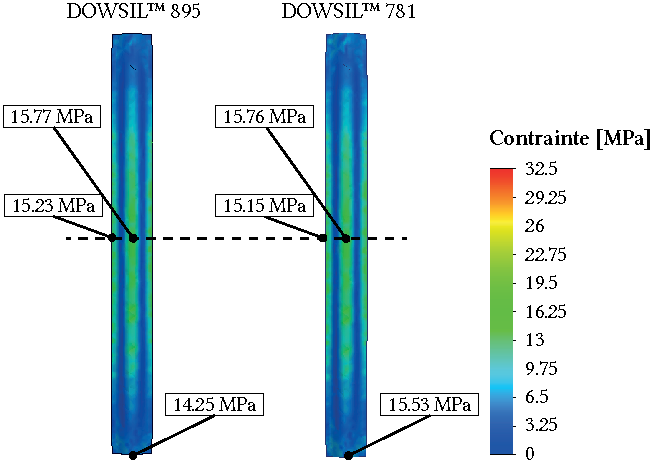
\includegraphics[width=\linewidth]{img/ondul/fem/femjoint3.pdf}
\caption{Calcul \acrshort{FEM} comparant les contraintes dans le verre selon le type de silicone (DOWSIL™ 895: haut module et DOWSIL™ 781: bas module).}
\label{fig:femjoints3}
\vspace{-10pt}
\end{wrapfigure}

On peut dès lors comparer l'impact de la rigidité du silicone sur la contrainte dans le verre en mettant en parallèle un silicone haut module d'élasticité (c'est le cas du DOWSIL™ 895) et un bas module d'élasticité (c'est le cas du DOWSIL™ 781). Cette comparaison est présentée dans la figure \ref{fig:femjoints3}. 
Comme attendu, la plus faible rigidité du DOWSIL™ 781 va engendrer plus de contraintes en pied et en tête du vitrage et une diminution de la contrainte sur les bords à mi-portée. La contrainte au niveau du creux du verre à mi-portée reste semblable. Cependant, la contrainte augmente, en pied, de près de 9\% avec le silicone DOWSIL™ 781 tandis qu'elle ne diminue que de 0.5\% à mi-portée. On comprend donc qu'il est préférable d'avoir un silicone très rigide pour empêcher le déplacement en pied et en tête du vitrage et donc une concentration des contraintes dans cette zone.

\subsubsection{Dimensionnement d'un vitrage autoportant en verre ondulé}
On peut désormais conclure en calculant l'épaisseur de verre minimale pour la réalisation de notre vitrage autoportant présenté dans la partie \ref{sec:temoin}.

\paragraph{Prédimensionnement de l'ondulation}\mbox{}

On cherche à diviser notre verre en 1, 2 ou 3 ondes sinusoïdales. L'équation (\ref{eq:s_maxondul}), modifiée pour correspondre au cas de charge à l'\acrshort{ELU}, permet un prédimensionnement de la hauteur de l'onde dans chacun des cas. La figure \ref{fig:sin_predim} présente le calcul de prédimensionnement ainsi que le schéma des trois périodes d'ondulation considérées. 

Si l'on regarde dans chaque cas la hauteur d'onde donnant le minimum de contrainte dans le verre, on observe que pour une épaisseur de verre donnée, celle-ci est quasiment identique quelque soit la période d'ondulation. Naturellement, la contrainte diminue lorsque l'épaisseur de verre augmente.

Pour comparer les périodes d'ondulation, on peut s'intéresser à la quantité de verre utilisée, c'est-à-dire la section de verre, pour obtenir ce minimum de contrainte, selon l'épaisseur du verre. Comme on pouvait s'y attendre, le cas à 3 ondes nécessite une plus grande section que le cas à 2 ondes, qui lui même nécessite une plus grande section que le cas à 1 onde. Plus l'épaisseur du verre augmente, plus cet écart de section augmente, allant de +11\% à +43\% entre la section à 2 ondes et celle à 1 onde et de +43\% à +233\% entre la section à 3 ondes et celle à 1 onde.

C'est la situation inverse pour la contrainte minimum pour une épaisseur de verre donnée. Toutefois, l'augmentation des contraintes par rapport au cas à 1 onde ne va que de +4\% à +10\% pour 2 ondes et de +10\% à +20\% pour 3 ondes.

En d'autres termes, pour une contrainte limite, une épaisseur de verre plus importante sera nécessaire dans le cas à 1 onde mais la quantité de verre nécessaire sera au final moindre. Cela concorde avec nos remarques relatives à la figure \ref{fig:ondulfem1}: si la longueur d'onde est trop petite par rapport à la hauteur de l'onde, le gain en inertie ne sera pas suffisamment important pour contrebalancer la perte en matière.

\begin{figure}[H]
    \centering
    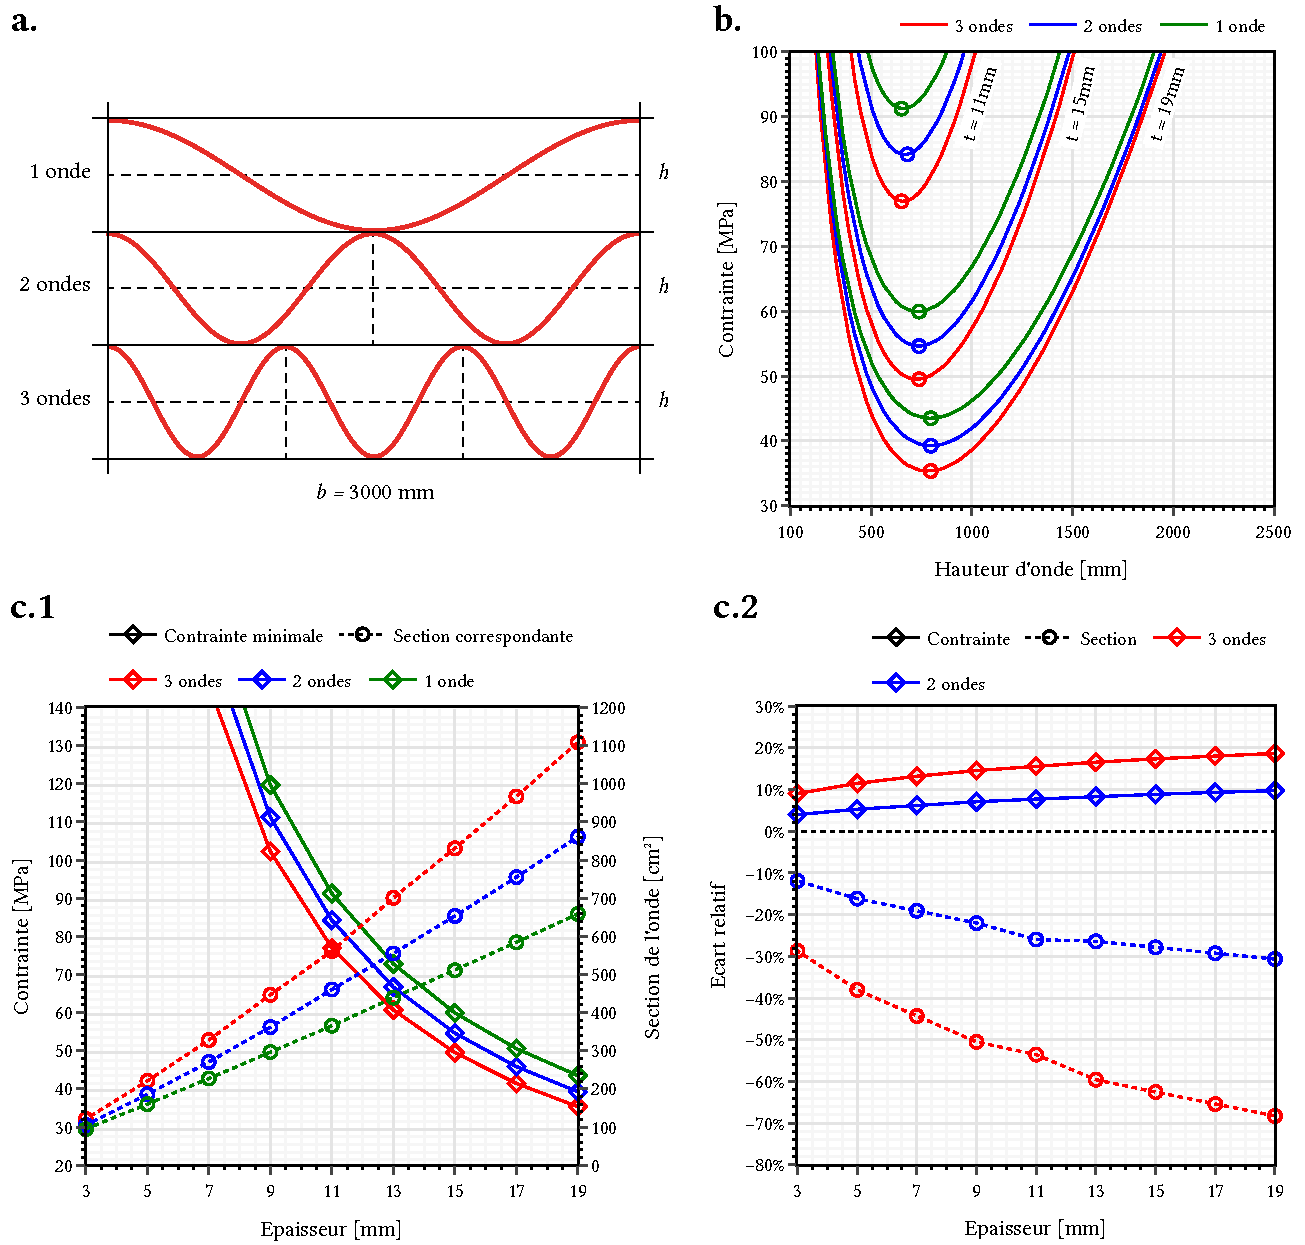
\includegraphics[width=\linewidth]{img/ondul/predim.pdf}
    \caption{\textbf{a.} Schémas des trois périodes d'ondulation considérée. \textbf{b.} Contrainte maximale dans le verre calculée d'après (\ref{eq:s_maxondul}) selon la hauteur de l'onde pour les trois périodes d'ondulation et l'épaisseur de verre. \textbf{c.} Comparaison des contraintes et des sections obtenus en prenant la hauteur d'onde minimisant la contrainte pour les trois cas, en fonction de l'épaisseur de verre (\textbf{1.} contrainte et section en fonction de l'épaisseur et \textbf{2.} écart relatif $\sigma_{\text{ER}} = \frac{\sigma_{\text{1 onde}}-\sigma_{\text{i ondes}}}{\sigma_{\text{1 onde}}}$ et $S_{\text{ER}} = \frac{S_{\text{1 onde}}-S_{\text{i ondes}}}{S_{\text{1 onde}}}$).}
    \label{fig:sin_predim}
\end{figure}
On obtient donc les épaisseurs et les sections de verre présentées dans le tableau \ref{tab:mat_predimsin} pour le verre durci et le verre trempé. La section de verre nécessaire est donc bien plus faible pour 1 onde que pour 2 ou 3 ondes mais la hauteur d'onde est l'épaisseur de verre sont plus importants. 

\begin{table}[H]
\centering
\caption{Épaisseur et section de verre minimum nécessaire pour le prédimensionnement.}
\label{tab:mat_predimsin}
\begin{tabularx}{\textwidth}{l*{5}{Y}}
\toprule
\textbf{Matériau} & \textbf{Limite d'élasticité}$f_y$ [\unit{\mega\pascal}] &\textbf{Nombre d'ondes} & \textbf{Épaisseur} $t$ [\unit{\milli\metre}]& \textbf{Hauteur d'onde} $h$ [\unit{\milli\metre}] & \textbf{Section} $S$ [\unit{\square\centi\meter}] \\\midrule
Verre durci & 45 & 1 onde & 18.5 &790& 640 \\
 & & 2 ondes & 17.25 &770& 770 \\
 & & 3 ondes & 16.1 & 755&900 \\
Verre trempé & 70 & 1 onde & 13.5 &715& 460 \\
 & & 2 ondes & 12.6 & 697&540 \\
 & & 3 ondes & 11.9 & 680&625 \\
\bottomrule
\end{tabularx}
\end{table}
Bien qu'on veuille diminuer l'épaisseur des vitrages, on souhaite avant tout économiser de la matière. On choisit donc un verre ondulé formé d'une seule onde de \qty{3}{\metre} de longueur d'onde et de \qty{790}{\milli\metre} de hauteur d'onde pour le verre durci et \qty{715}{\milli\metre} pour le verre trempé.

\paragraph{Calcul de l'épaisseur de verre minimale}\mbox{}

Comme nous l'avons vu précédemment, le calcul analytique sous-évalue les contraintes dans le verre. De plus notre vitrage autoportant a vocation à être la composante d'un mur rideau de plusieurs vitrages. Il est donc nécessaire de dimensionner plus précisemment le vitrage en effectuant un calcul \acrshort{FEM} prenant en compte plusieurs vitrages comme on a pu le faire dans le calcul présenté dans la figure \ref{fig:femjoints}.

On effectue donc un calcul \acrshort{FEM} pour un ensemble constitué de 7 panneaux de verre ondulé aux dimensions déterminées précédemment, pour différentes épaisseurs.
\begin{figure}[H]
    \centering
    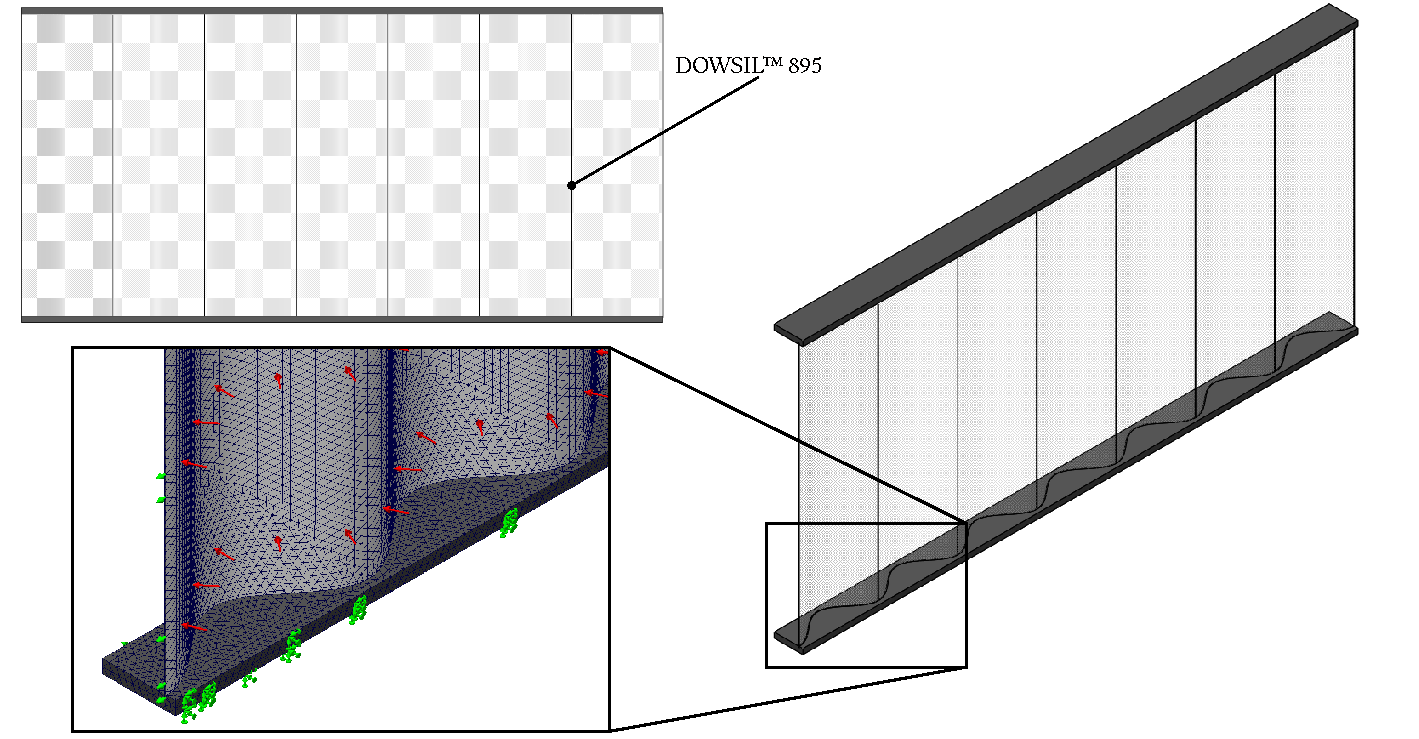
\includegraphics[width=\linewidth]{img/ondul/fem/dim_fem.pdf}
    \caption{Géométrie et maillage SOLIDWORKS du verre ondulé pour son dimensionnement.}
    \label{fig:dim_onful_model}
\end{figure}

Les résultats des calculs \acrshort{FEM} sont présentés dans la figure \ref{fig:dim_onful_float}. On observe que la contrainte maximale sur l'ensemble des panneaux de verre est situé dans le verre aux extrémités du modèle. Cependant, afin de simuler un très grand nombre de vitrages, on ne s'intéresse qu'à la contrainte dans le verre central.

\begin{figure}[H]
    \centering
    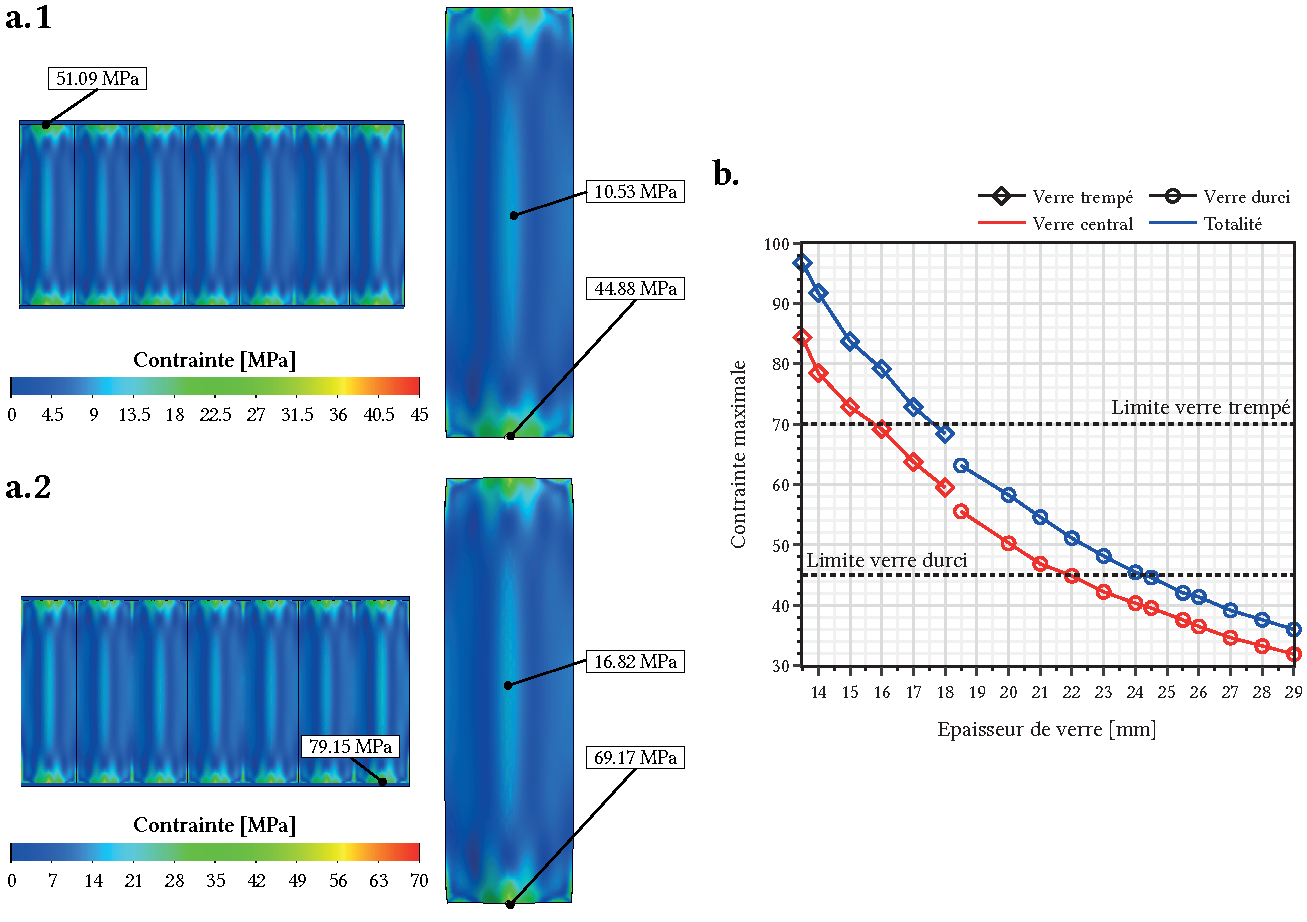
\includegraphics[width=\linewidth]{img/ondul/fem/dim_float.pdf}
    \caption{\textbf{a.} Résultats du dimensionnement du verre ondulé par calcul \acrshort{FEM} pour \textbf{1.}. le verre durci et \textbf{2.} le verre trempé. \textbf{b.} Contraintes maximales dans le verre selon son épaisseur pour le verre durci et trempé.}
    \label{fig:dim_onful_float}
\end{figure}

On obtient ainsi pour le verre durci une épaisseur minimale de \qty{22}{\milli\meter} (section de verre de \qty{761.08}{\centi\square\meter}), engendrant une contrainte maximale dans le verre de $\qty{44.88}{\mega\pascal} < f_y = \qty{45}{\mega\pascal}$. Pour le verre trempé, on obtient \qty{16}{\milli\meter} (section de verre de \qty{454.18}{\centi\square\meter}) pour une contrainte maximale dans le verre de $\qty{67.17}{\mega\pascal} < f_y = \qty{70}{\mega\pascal}$ .

\subsubsection{Conclusion sur le verre ondulé}

Nous avons réussi, notamment en considérant la collaboration entre les vitrages de la façade, à réduire considérablement la quantité de verre nécessaire à la réalisation d'un vitrage autoportant grâce à un vitrage ondulé. 

Nous avons pu observer que la forme des ondulations mais aussi la taille de ces ondulations avaient une grande importance pour réduire la quantité de verre. 

L'étude de la collaboration entre les vitrages a permis de soulever des questions importantes, notamment sur le comportement aux extrémités du vitrage qui mériterait une étude plus poussée. On pourrait par exemple envisager d'ajouter des cales plus rigides en pied et en tête entre les vitrages pour obtenir une plus grande rigidité et réduire la flexion dans ces parties du verre, ou encore envisager de retirer un morceau de verre au milieu de ces parties afin de permettre le mouvement du verre et empêcher le flexion.

\newpage
\subsection{Cintrage du verre à froid}

Le verre ondulé ayant prouvé son efficacité, on peut s'intéressser à des formes de verre plus libres, en considérant de la double courbure plutôt que de la simple courbure comme avec le verre ondulé.

En effet, rajouter de la courbure dans l'autre sens pourrait permettre de répartir de manière plus homogène les contraintes mécaniques.

Il existe plusieurs techniques pour courber le verre tels que le cintrage à chaud ou le cintrage à froid. Le cintrage à froid étant la technique la plus simple et la plus économique, on choisit ici d'étudier les bénéfices possibles d'un verre cintré à froid. 


\begin{figure}[H]
    \centering
    \includegraphics[height=0.327\textwidth]{img/cintrage_froid/BahnshofStrassburg_c_Reithmeier__1_.jpg}\hfill
    \includegraphics[height=0.327\textwidth]{img/cintrage_froid/BahnhofStrassburg_c_Obertreis__2_.jpg}
    \\[\smallskipamount]
    \includegraphics[height=0.465\textwidth]{img/cintrage_froid/ChadstoneSC_05.jpg}\hfill
    \includegraphics[height=0.465\textwidth]{img/cintrage_froid/ChadstoneSC_09.jpg}\hfill
    \caption{Photographies de la façade en verre cintré à froid de la Gare de Strasbourg, par \Textcite{GareStrasbourg} (première ligne) et du Chadstone Shopping Center, par \Textcite{chadstone1} et \Textcite{chadstone2} (seconde ligne).}
    \label{fig:cintragefroidphoto}
\end{figure}
Cette technique est d'ailleurs de plus en plus utilisé dans la construction afin de concevoir des façades à géométries complexes de façon plus économique qu'avec du cintrage à chaud. Le cintrage à froid permet également de conserver les propriétés optiques du verre qu'on pourrait perdre par cintrage à chaud. La figure \ref{fig:cintragefroidphoto} présente deux exemples de façades réalisés avec des panneaux de verres cintrés à froid. Il est à noter que cette technique nécessite généralement l'utilisation de verres plus épais que si l'on chauffait à chaud.
\\

Afin d'étudier les bénéfices possibles d'un vitrage à double courbure cintré à froid, on doit en premier lieu déterminer les formes admissibles par cintrage à froid. En général on déforme le verre pour le fixer à un cadre linéaire ou courbe et les formes prises par le verre sont limités par la théorie.
\begin{figure}[H]
    \centering
    \includegraphics[width=0.75\textwidth]{img/cintrage_froid/fig4_74.jpg}
    \caption{Formes les plus couramment utilisées par cintrage à froid, d'après \Textcite{meinhardt}.}
    \label{fig:cintragefroidtypes}
\end{figure}

Nous étudierons donc dans un premier temps les formes possibles de verre cintré à froid d'après la théorie simple des petites déformations puis nous regarderons le cas réel et nous finirons par une étude d'un verre autoportant cintré à froid afin de déterminer si les formes obtenus peuvent être bénéfiques.

\subsubsection{Théorie des petites déformations}
Pour étudier le cintrage à froid des panneaux de verre on peut commencer par étudier la théorie la plus simple: la théorie des petites déformations des plaques minces (théorie de Kirchoff). On fait donc les hypothèses suivantes (d'après \Textcite{mcst2}):
\begin{itemize}
    \item Le matériau (ici  le verre) est homogène, isotropique et élastique linéaire;
    \item La plaque est initiallement plane;
    \item Le plan moyen de la plaque ne subit pas d'allongement ou de contraction pendant le chargement;
    \item L'épaisseur de la plaque est petite comparée aux autres dimensions ($t < \text{min}(L,l)/10$);
    \item La déformation de la plaque $w(x,y)$ est petite comparée à l'épaisseur de la plaque ($w < t/10$) et les pentes ou angles de roation sont petits devant l'unité;
    \item L'hypothèse de Navier-Bernoulli reste valable: les sections planes restent planes après déformations et perpendiculaires au plan moyen déformé;
    \item Les déformations dues à l'effort tranchant sont négligées;
    \item Les contraintes $\sigma_{zz}$ dans la direction transverse sont négligeables par rapport aux contraintes $\sigma_{xx}$ et $\sigma_{yy}$.
\end{itemize}

\begin{figure}[H]
    \centering
    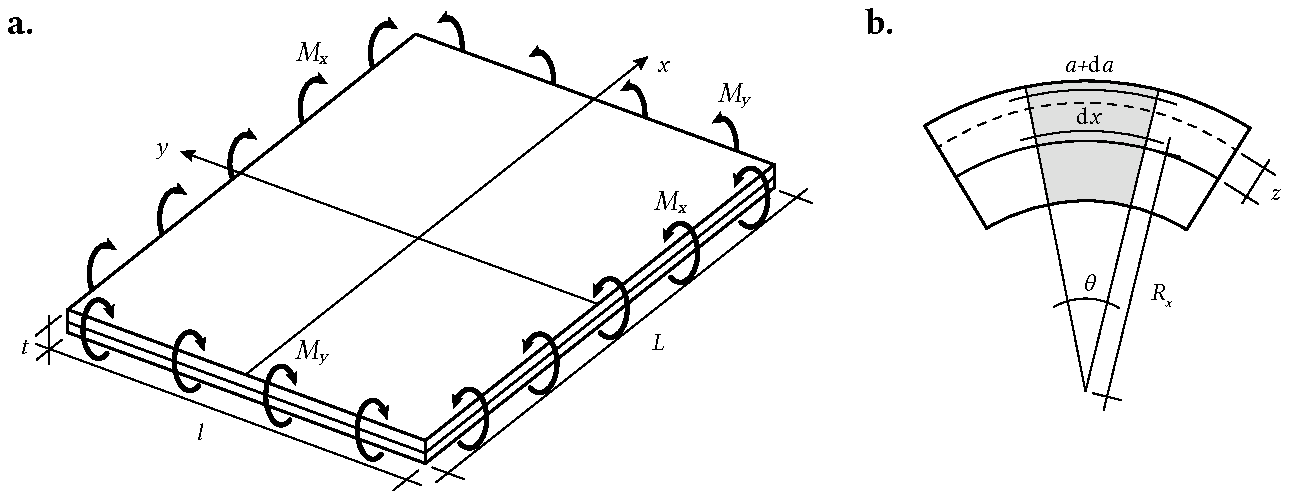
\includegraphics[width=\textwidth]{img/cintrage_froid/petitedef.pdf}
    \caption{\textbf{a.} Schéma de la plaque mince en flexion pure. \textbf{b.} Section de plaque considérée dans la direction $x$.}
    \label{fig:petite_def}
\end{figure}

On étudie une plaque de longueur $L$, de largeur $l$ et d'épaisseur $t$ en flexion pure, c'est-à-dire soumis à des moments linéiques $M_x$ et $M_y$ le long de ses bords de direction $x$ (longueur $L$) et $y$ (largeur $l$). On cherche à calculer la contrainte dans cette situation. On base nos calculs sur l'ouvrage de \Textcite{timo_plaque}.

Une section de la plaque dans un plan normal à l'axe $y$ (section de direction $x$) va se courber sous l'effet de la flexion. On peut alors calculer l'élongation et la contraction de ses fibres via son rayon de courbure $R_x$ donné par:
\begin{align}
    \theta = \frac{\mathrm{d}x}{R_x} = \frac{a+\mathrm{d}a}{z+R_x}
\end{align}
sous l'hypothèse que sa fibre neutre ni ne s'allonge ni ne se rétracte. Alors:
\begin{align}
    \mathrm{d}a = \frac{z\mathrm{d}x}{R_x}
\end{align}
On en déduit la déformation dans la direction $x$, et par la même occasion dans la direction $y$:
\begin{align}
    \varepsilon_x &= \frac{\mathrm{d}a}{a} = \frac{z}{R_x}\\
    \varepsilon_y &= \frac{\mathrm{d}a}{a} = \frac{z}{R_y}
\end{align}
On rappelle la loi de Hooke pour une plaque:
\begin{align}
    \varepsilon_x &= \frac{1}{E}\left ( \sigma_x - \nu \sigma_y \right )\\
    \varepsilon_y &= \frac{1}{E}\left ( \sigma_y - \nu \sigma_x \right )
\end{align}
Ce qui nous permet de calculer les contraintes dans la plaque:
\begin{align}
    \sigma_x &= \frac{E}{1-\nu^2}z\left (\frac{1}{R_x} + \nu \frac{1}{R_y}\right )\label{eq:cintragex}\\
    \sigma_y &= \frac{E}{1-\nu^2}z\left (\frac{1}{R_y} + \nu \frac{1}{R_x}\right ) \label{eq:cintragey}
\end{align}
Dans la suite on notera les courbures de la plaque $K_x = \frac{1}{R_x}$ et $K_y = \frac{1}{R_y}$. 

On peut ainsi calculer les moments linéique dans la section de la plaque:
\begin{align}
    M_x &= \int_{-t/2}^{t/2} \sigma_x z \mathrm{d}z = D \left (K_x + \nu K_y\right )\\
    M_y &= \int_{-t/2}^{t/2} \sigma_y z \mathrm{d}z = D \left (K_y + \nu K_x\right )
\end{align}
où $D = \frac{Et^3}{1-\nu^2}$ est la rigidité de la plaque. Cela nous permet de calculer la déformation de la plaque en utilisant les équations différentielles suivantes:
\begin{align}
\frac{\partial^2w}{\partial x^2} &= -K_x \\
\frac{\partial^2w}{\partial y^2} &= -K_y
\end{align}
Ainsi, en plaçant l'origine du repère au centre de la plaque et que le plan tangent à la surface de la plaque en ce point reste horizontal, on obtient l'équation d'un paraboloïde:
\begin{align}
w(x,y)  = -\frac{M_x - \nu M_y}{2D(1-\nu^2)} x^2 - \frac{M_y - \nu M_x}{2D(1-\nu^2)} y^2
\end{align}

\begin{figure}[H]
    \centering
    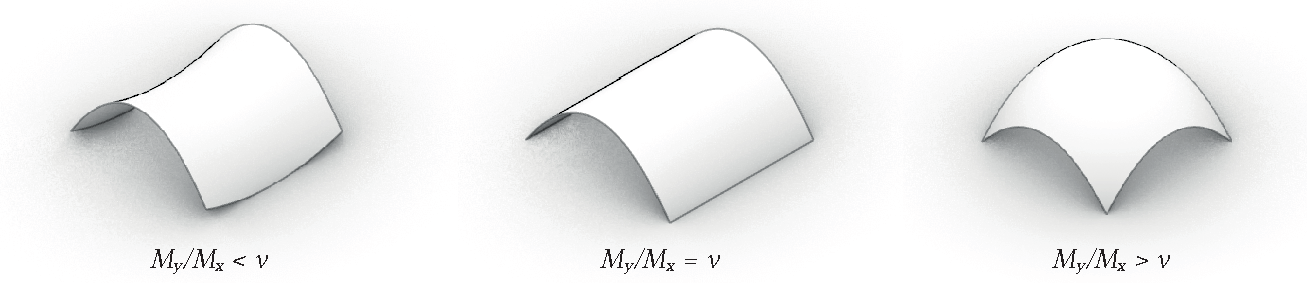
\includegraphics[width=\textwidth]{img/cintrage_froid/shapes.pdf}
    \caption{Formes prises par la plaque en flexion pure ($M_y < M_x$).}
    \label{fig:petite_def}
\end{figure}

\subsubsection{Limites géométriques en petites déformations}

La théorie des petites déformations impose donc l'espace des formes obtenable par la mise en flexion pure d'une plaque. En effet, il n'est possible de réaliser que des paraboloïdes elliptiques (ce qu'on pourrait appeler vulgairement un "bout de dirigeable") ou des paraboloïdes hyperboliques (ce qu'on pourrait appeler vulgairement une "selle de cheval"). Il n'est donc, par exemple, pas possible d'obtenir des surfaces sphériques (bout de sphère) d'après la théorie des petites déformations.
\\

De plus, les équations (\ref{eq:cintragex}) et (\ref{eq:cintragey}) nous permettent d'obtenir des informations sur les courbures possibles de la plaque. En effet, on peut calculer les courbures extremales possibles sans rupture de la plaque. On s'intéresse pour cela à deux critères: le critère de Tresca et le critère de Von Mises.

Pour Tresca, le critère s'écrit simplement:
\begin{align}
\max\left ( \left | \sigma_x - \sigma_y\right |,\left | \sigma_x\right |,\left | \sigma_y\right |\right ) \leq f_y
\end{align}

Le critère de Von Mises sécrit quant à lui:
\begin{align}
\sqrt{\sigma_x^2+\sigma_y^2-\sigma_x\sigma_y} \leq f_y
\end{align}

En traçant la frontière du domaine de ces deux critères en fonction des courbures de la plaque on peut remarquer que la courbure obtenu par la flexion pure de la plaque est limitée. Comme attendu, le critère de Tresca, plus simple, offre moins de possibilités pour les courbures. 

\begin{wrapfigure}{l}{0.45\textwidth}
    \vspace{-10pt}
    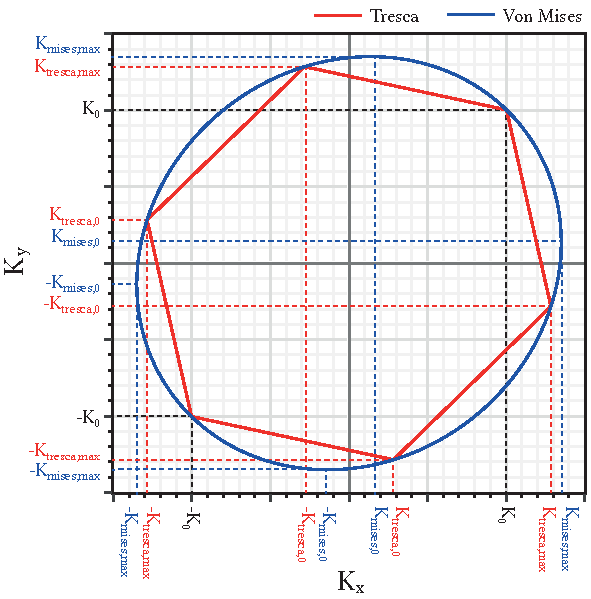
\includegraphics[width=\linewidth]{img/cintrage_froid/critere_petitedef.pdf}
       \caption{Schéma du critère de Tresca et de Von Mises en fonction des courbures $K_x$ et $K_y$ de la plaque.}
   \label{fig:tresca_mises}
   \end{wrapfigure}

Selon le critère de Tresca, on peut obtenir une plus forte courbure de la plaque en cherchant une forme à double courbure négative ($K_x/K_y < 0$). Dans ce cas, la courbure maximale dans un sens est égale à:
\begin{align}
K_{\text{tresca,max}} = \frac{f_y}{Et/2}
\end{align}
On aura alors une courbure plus faible dans l'autre sens égale à:
\begin{align}
    -K_{\text{tresca,0}} = \frac{-\nu f_y}{Et/2}
\end{align}
Le critère de Von Mises permet d'obtenir une plus grande courbure avec de la double courbure positive ($K_x/K_y > 0$). Avec ce critère la courbure maximale dans un sens est:
\begin{align}
K_{\text{mises,max}} = \frac{f_y}{Et/2}\times 2\sqrt{\frac{1-\nu+\nu^2}{3}}
\end{align}
Dans ce cas, la courbure dans l'autre sens vaudra:
\begin{align}
    K_{\text{mises,0}} = \frac{f_y}{Et/2}\times \frac{1-4\nu+\nu^2}{\sqrt{3(1-\nu+\nu^2)}}
\end{align}

On peut soulever une dernière situation remarquable: la courbure maximale lorsque que les courbures dans les deux sens sont égales (donc en double courbure positive) est la même pour les deux critères et est égale à:
\begin{align}
    K_0 = \frac{f_y}{Et/2}\times (1-\nu)
\end{align}

On peut effectuer une rapide application numérique pour un verre durci de \qty{10}{\milli\metre} d'épaisseur. La courbure maximale admise par le critère de Von Mises est alors de \qty{0.131}{\per\metre}. Cela correspond à une flèche de \qty{18}{\milli\metre} sur une plaque de \qty{1}{\metre} de long, soit une flèche de l'ordre de $L^2/55$. A noté que la flèche obtenue est inversement proportionnelle à l'épaisseur du verre. Ainsi, en passant, par exemple, à un verre de \qty{5}{\milli\metre} d'épaisseur on peut atteindre une flèche de \qty{36}{\milli\metre}.

Toutefois, pour rester dans le domaine des hypothèses de la théorie des petites déformations, il faut que la déformation soit plus petite que le dixième de l'épaisseur de la plaque. On peut relier cette hypothèse à la courbure et obtenir que la courbure de la plaque doit respecter l'inégalité suivante:
\begin{align}
K_{\text{max}} < \frac{2t}{5L^2}
\end{align}
Ce qui, pour une plaque en verre durci de \qty{10}{\milli\metre} d'épaisseur et de \qty{1}{\metre} de long, impose que la courbure ne dépasse pas \qty{0.004}{\per\metre}, ce qui est près de 30 fois moins que la courbure maximale admise par le critère de Von Mises. Mais en pratique, on réussit tout de même à obtenir de la double courbure et des formes se rapprochant de paraboloïdes par cintrage à froid avec de grandes déformations. Il faut donc pousser la théorie plus loin pour être dans le domaine de validité qui nous intéresse.

\subsubsection{Cas réel: flambement des plaques}

Comme dit précédemment, on peut observer des formes se rapprochant de paraboloïdes lorsque l'on cintre du verre à froid. Toutefois \Textcite{staaks}, remarque, en observant la distorsion optique du verre, que la forme attendue par la théorie des petites déformations n'est pas celle réellement produite.

En réalité, une plaque mise en flexion en grandes déformations va vouloir conserver une forme développable (donc à simple courbure). 

Si l'on prend le cas de la torsion par cintrage à froid du verre (c'est-à-dire le cas où $K_x = -K_y$, ou encore $M_x = -M_y$), l'expérience montre que le verre passe par deux modes de déformation lorsque l'on augmente la déformation. Un premier dans lequel le verre prend la forme d'un paraboloïde hyperbolique. Puis un second mode où la déformation ne va plus être symétrique et la plaque va tendre vers une forme à simple courbure. \Textcite{buckling_cold}, expliquent que ce second mode correspond au flambement du verre. Une diagonale va alors se rigidifier tandis que l'autre va gagner en courbure. Les bords de la plaque ne restent alors pas droits mais se courbent. Ils obtiennent, pour une plaque de verre de \qtyproduct{2 x 2}{\metre} et de \qty{10}{\milli\metre} d'épaisseur, que ce changement de mode de déformation se produit lorsque le déplacement atteint environ \qty{40}{\milli\metre} (c'est-à-dire une distance verticale de \qty{80}{\milli\metre} entre deux coins successifs). Un tel déplacement engendre une courbure de \qty{0.04}{\per\metre}, ce qui est 10 fois supérieur à la limite de l'hypothèse des petites déformations. 

\Textcite{buckling_cold}, montrent par ailleurs que rigidifié les bords du verre avec un cadre rigide permet d'augmenter le déplacement limite avant le flambement de la plaque. 

On observe sur la figure \ref{fig:non_linear_cintr2} que le calcul linéaire statique du cintrage sous-évalue les contraintes résiduelles dans le verre. \Textcite{buckling_cold}, expliquent que les grandes déformations entraônent de grandes contraintes membranaires dans le plan médian de la plaque ce qui est négligé dans la théorie linéaire. Il est donc nécessaire dans la suite d'effectuer des calculs non linéaires, bien qu'ils soient plus complexes, afin de ne pas sous-évaluer les contraintes dans le verre. 
\begin{figure}[H]
    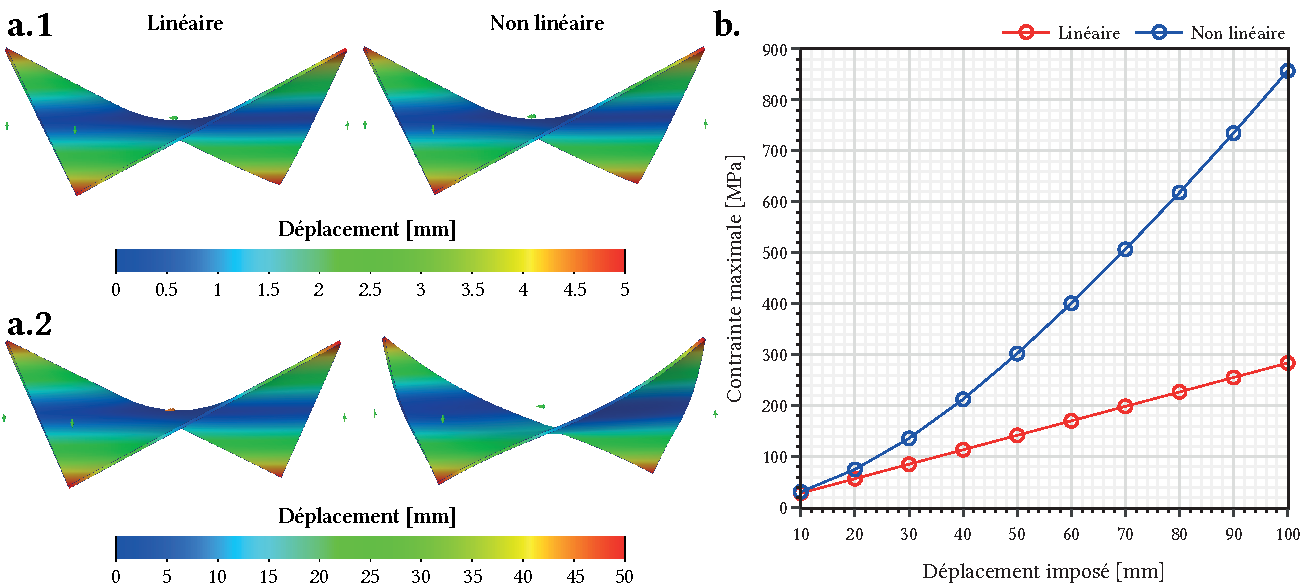
\includegraphics[width=\linewidth]{img/cintrage_froid/non_linear2.pdf}
       \caption{\textbf{a.} Déformations linéaires et non linéaires sous l'effet d'un déplacement vertical imposé à deux coins opposés (\textbf{1.} $\delta = \qty{10}{\milli\metre}$, \textbf{2.} $\delta = \qty{100}{\milli\metre}$); \textbf{b.} contraintes maximales, calculées par une analyse FEM linéaire et non linéaire, selon le déplacement imposé; plaque de verre carré de \qtyproduct{1 x 1}{\metre} de \qty{10}{\milli\metre} d'épaisseur.}
   \label{fig:non_linear_cintr2}
   \end{figure}
\subsubsection{Étude d'un verre autoportant cintré à froid}

\begin{wrapfigure}{l}{0.3\textwidth}
    \vspace{-10pt}
    \centering
    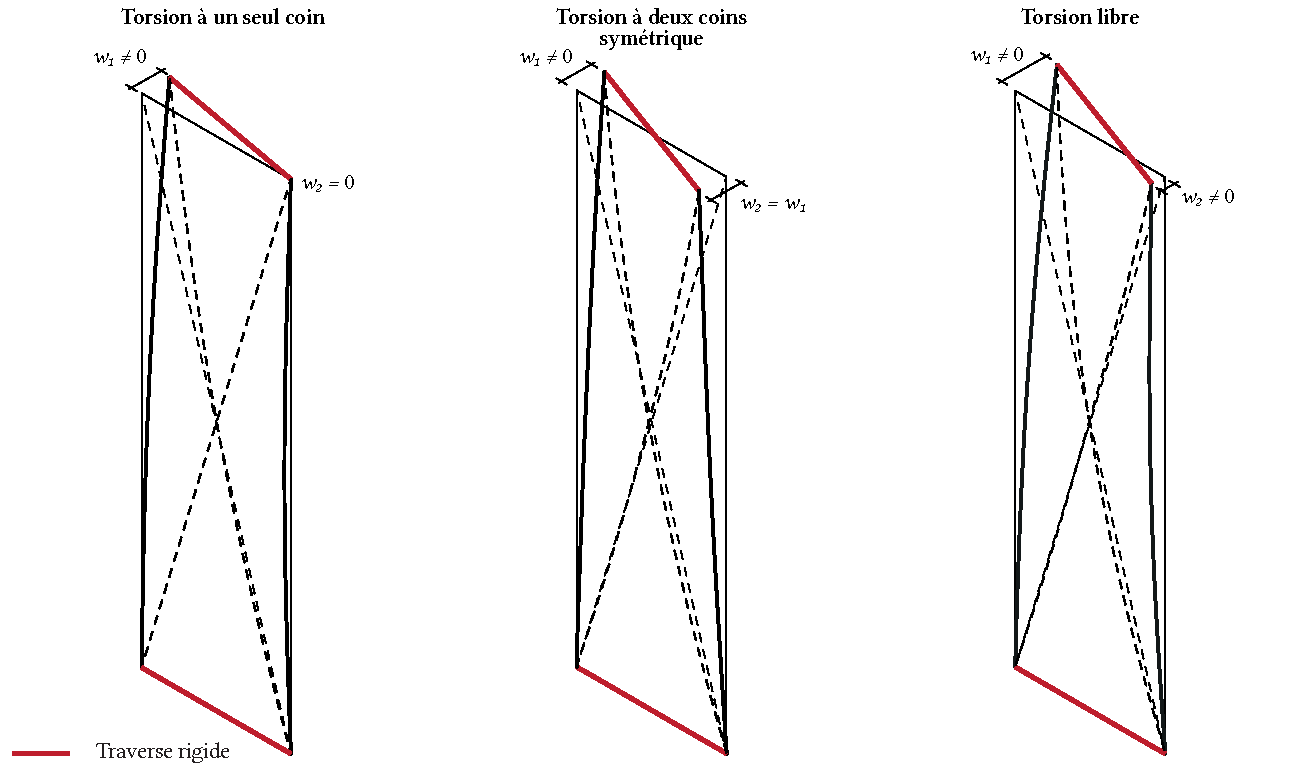
\includegraphics[width=0.7\linewidth]{img/cintrage_froid/def.pdf}
       \caption{Schéma du cintrage à froid considéré.}
   \label{fig:forme_cintr}
   \end{wrapfigure}

Dans notre étude nous nous intéressons exclusivement aux panneaux de verre autoportants. Mais dans ce cas il n'est pas possible d'encadrer le verre sur ses quatres bords puisque cela va à l'encontre du principe de verre autoportant. Ainsi on s'intéresse au cas particuluer où seuls les bords en pied et en tête du vitrage sont encadrés par des traverses rigides. On s'intéresse aux formes obtenus par cintrage à froid en faisant pivoter la traverse supérieure comme schématisé dans la figure \ref{fig:forme_cintr}. Dans ce cas, les bords supérieurs et inférieurs du verre restent droits grâce aux traverses mais les bords latéraux se courbent sous l'effet du déplacement imposé. 

La forme obtenue dépend alors du déplacement $w_1$ imposé à un des coins. Cette déformation engendre des contraintes dans le verre que l'on peut observer dans la figure \ref{fig:cintrage_twist}. Comme attendu, ces contraintes sont croissantes de l'épaisseur du verre et du déplacement imposé. La contrainte maximale dans le verre se situe en tête et en pied du verre.
\begin{figure}
    \centering
    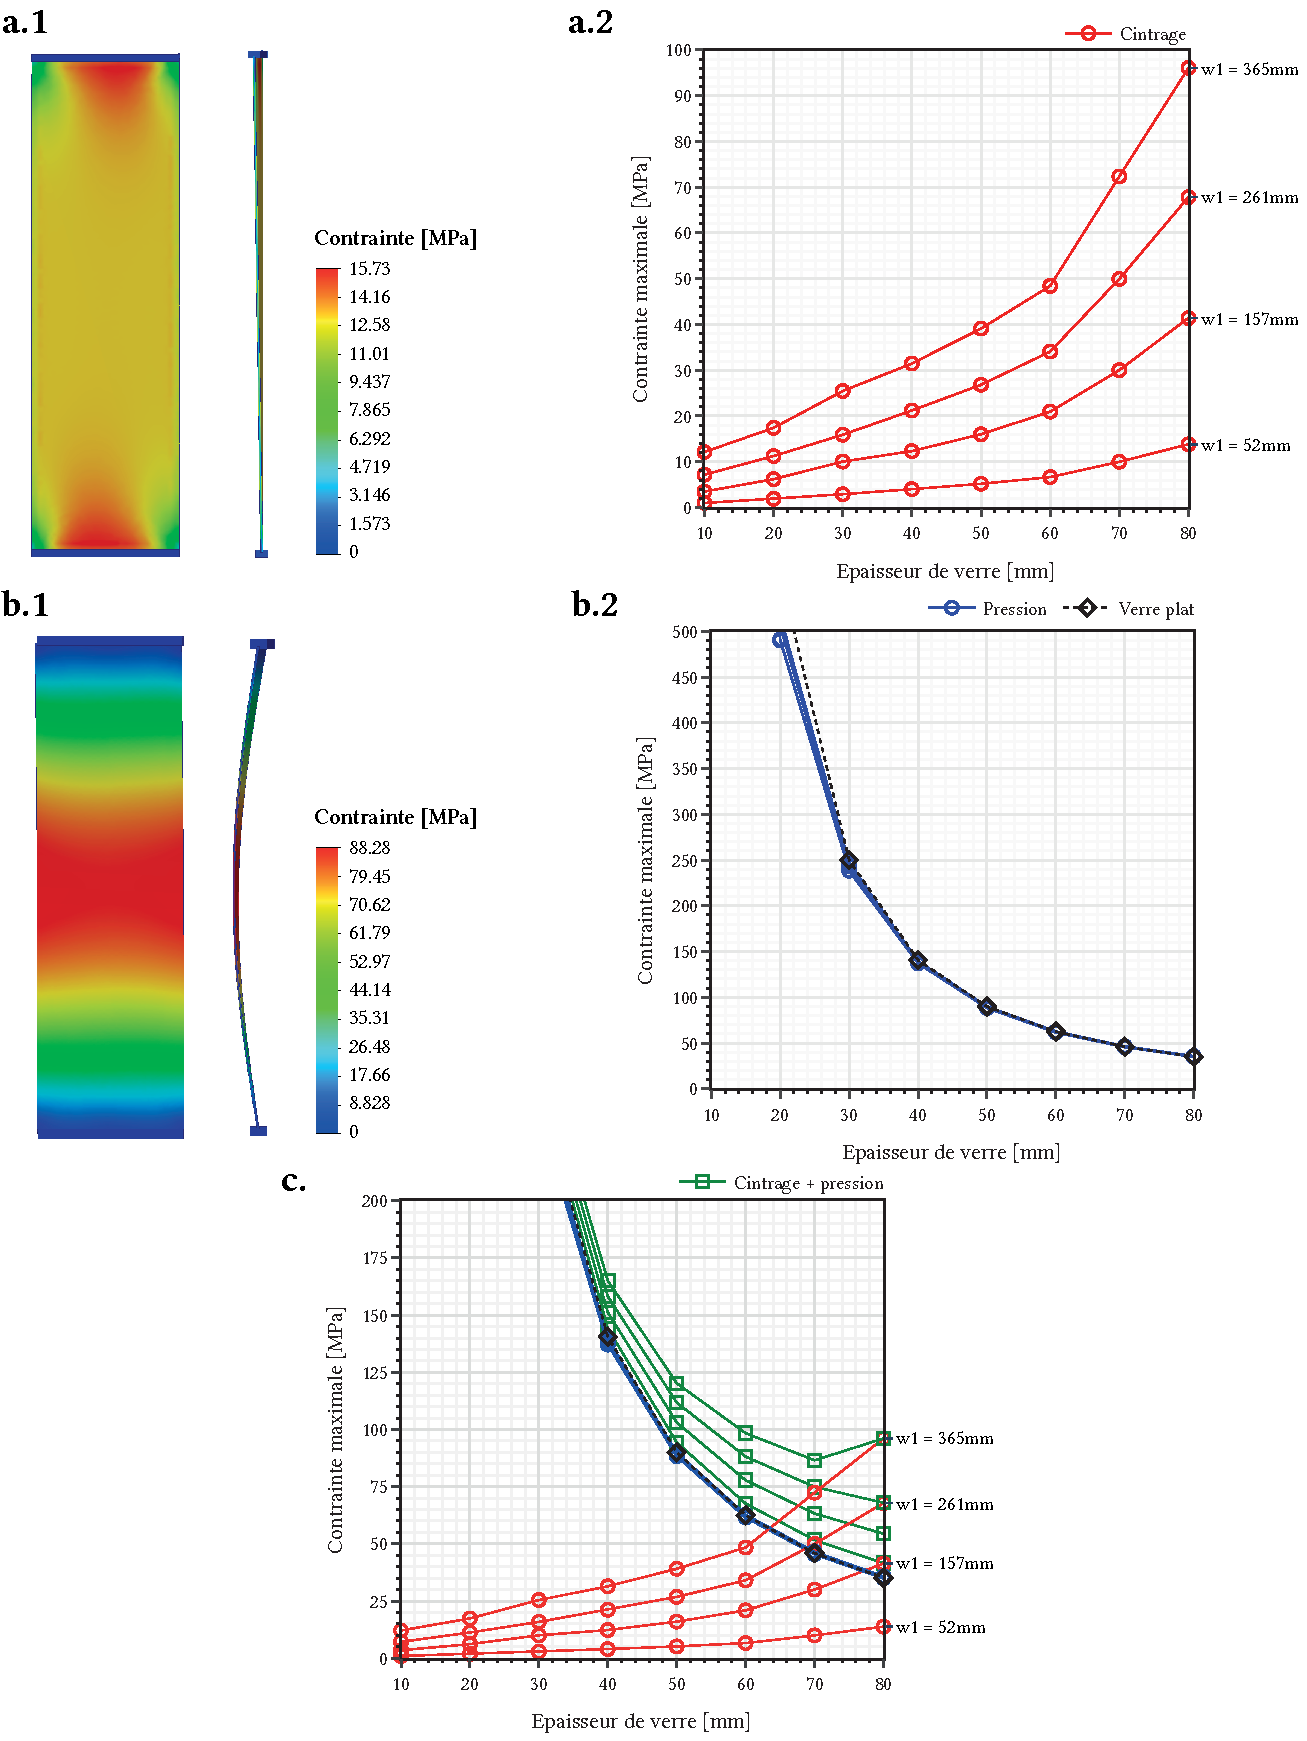
\includegraphics[width=0.98\textwidth]{img/cintrage_froid/twist.pdf}
    \caption{Contrainte maximale dans le verre selon son épaisseur pour différents déplacements $w_1$ imposés (\textbf{a.} cintrage, \textbf{b.} pression de vent sur le verre déformée sans les contraintes du cintrage et \textbf{c.} contraintes totales dans le verre).}
    \label{fig:cintrage_twist}
\end{figure}
Si l'on prend le verre déformé et que l'on applique les chargements considérés dans notre étude, sans prendre en considération les contraintes déjà présentes engendrée par le cintrage, on observe que la contrainte calculée par éléments finis dans le verre est très proche du résultat analytique du verre plat. C'est d'autant plus vrai pour de grandes épaisseurs de verre. Ainsi en approximant la contrainte au résultat analytique :
\begin{align}
\frac{3P z (10 -z)}{t^2}
\end{align}
 où $z$ est l'atitude du point auquel on calcul la contrainte sur le verre; on peut calculer la contrainte totale en tout point du verre en sommant simplement avec la contrainte de cintrage. 

 On obtient naturellement que la contrainte totale dans le verre est toujours supérieur à la contrainte maximale dans un verre plat de même épaisseur. 
\\

Pour s'écarter du résultat du verre plat on peut essayer d'augmenter la déplacement imposé pour augmenter la courbure du verre et profiter de sa forme. Cependant en regardant dans les détails, on observe que la forme obtenue par ce procédé n'est pas favorable puisque la contrainte engendrée par la pression de vent augmente selon le déplacement imposé. 
\subsubsection{Conclusion sur le verre cintré à froid}

Ainsi il ne semble pas pertinent de considérer le cintrage à froid pour obtenir de la double courbure dans notre vitrage autoportant. En effet, les contraintes engendrées dans le verre par le cintrage deviennent trop importantes à mesure que l'on déforme le vitrage. 

Le critère autoportant du vitrage, c'est-à-dire l'absence de meneaux verticaux, limite les formes de verres possibles. Cependant nous avons choisis ici de simplement déplacer un coin du vitrage. Il pourrait être intéressant de cintrer le verre en le fixant sur des traverses courbes afin d'obtenir une forme s'approchant d'un bout de sphère. 

\newpage
\subsection{Le verre bulle}

Introduction sur le Vakko HQ et lien avec le verre ondulé. 

\begin{figure}[H]
    \centering
    \includegraphics[height=0.324\linewidth]{img/bulle/Vakko_ext2.jpg}\hfill
    \includegraphics[height=0.324\linewidth]{img/bulle/Vakko_ext.jpg}
    \\[\smallskipamount]
    \includegraphics[width=\linewidth]{img/bulle/Vakko_int.jpg}
    \caption{Photographies de la façade du Vakko Headquarters and Power Media Center, par \Textcite{VekkoHQ}.}
    \label{fig:VakkoHQ}
\end{figure}

La volonté architecturale de REX pour le Vakko Headquarters a été de mettre en valeur une ancienne structure en béton plutôt que de la cacher. Pour cela ils ont voulu réaliser une façade en verre très mince afin qu'elle soit le plus transparent possible et ce sans cadre. Cette volonté architecturale a engendré un défi technologique: celui de concevoir une façade en verre mince sans meneaux. 

\begin{figure}[H]
    \centering
    \includegraphics[width=\linewidth]{img/bulle/stringio.jpg}
    \caption{Calcul de la façade su Vakko Headquarters and Power Media Center, par \Textcite{REX}. \textit{Sous-titre: L'insertion d'un X structurel dans chaque vitre permet d'augmenter la résistance du verre, d'éliminer le besoin de meaneaux aux bords et de réduire son épaisseur. (traduit de l'anglais)}}
    \label{fig:REXcalc}
\end{figure}

Pour cela ils ont renforcé le panneau de verre tenu ponctuellement en ajoutant un "X". D'après REX, ce "X" permet d'augmenter la résistance du verre malgré, ses maintiens ponctuels, et donc de réduire l'épaisseur du verre.
\\

On peut donc s'inspirer de ce principe dans le cadre de notre recherche autour de l'optimisation géométrique des panneaux de verre autoportant. Nous allons donc étudier le bénifice structurel d'une telle nervure mais aussi explorer les différentes formes de bulles possibles afin de déterminer s'il existe des formes plus ou moins optimales. 

\subsubsection{Etude préliminaire sur les formes de bulles}

On commence donc par s'intéresser aux formes de bulles possibles afin de déterminer la ou les meilleures formes pour optimiser notre épaisseur de verre. Les cas simples étudiés sont schématisés dans la figure \ref{fig:types_bulle}. 

\begin{figure}[H]
    \centering
    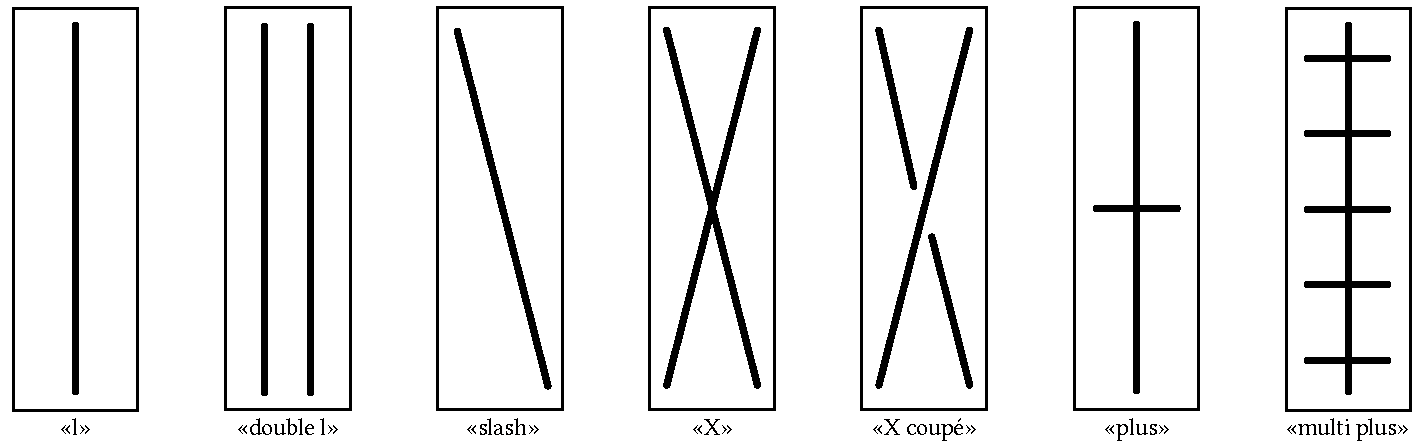
\includegraphics[width=\linewidth]{img/bulle/types_bulles.pdf}
    \caption{Géométries et nomenclature des bulles considérées.}
    \label{fig:types_bulle}
\end{figure}

Les lignes épaisses noires représentent la position de la bulle sur le verre. 

\begin{wrapfigure}{l}{0.3\textwidth}
    \centering
    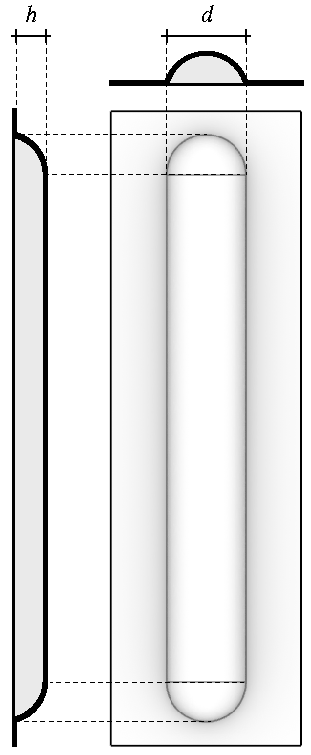
\includegraphics[width=0.8\linewidth]{img/bulle/geo_bulles1.pdf}
    \caption{Description de la géométrie d'une bulle.}
    \label{fig:geo_bulle1}
    \vspace{-10pt}
    \end{wrapfigure}

Pour cette approche simpliste on modélise la bulle par un bout de cylindre de diamètre $d$ dont l'axe est à une distance $d/2-h$ du vitrage. En dehors de la bulle, le vitrage est plat. L'épaisseur du verre est la même en tout point du vitrage. Cette modélisation est présentée dans la figure \ref{fig:geo_bulle1}.
\\

L'objectif va donc être, pour chaque forme de bulles, de déterminer les valeurs optimales de $h$ et $d$, c'est-à-dire donnant lieu à la plus faible épaisseur de verre. 

Pour cela on utilise l'outil paramétrique Karamba3D permettant de faire de rapides calculs \acrshort{FEM} via Grasshopper dans le logiciel de modélisation 3D Rhino3D. Afin de pouvoir préserver une cohérence des outils de calcul utilisés, on décide de comparer, sur un exemple de géométrie non simple, les résultats de SOLIDWORKS avec ceux de Karamba3D.

La figure \ref{fig:comp_kar} présente des résultats très similaires entre les deux logiciels de calcul. L'écart entre les contraintes maximales est bien plus grande pour de grandes contraintes que pour de faibles contraintes. Toutefois, Karamba3D est plus sensible au flambement que SOLIDWORKS. Ainsi, il pourrait être possible d'avoir des géométries flambant avec Karamba3D mais étant admissible avec SOLIDWORKS. Le calcul au second ordre de Karamba3D est d'ailleurs plus proche de celui de SOLIDWORKS que le premier ordre. Lorsqu'il n'y a pas de flambement, on peut observer que l'écart relatif de la contrainte maximale est inférieure à \qty{6}{\percent} pour le premier ordre et \qty{4}{\percent} pour le second ordre. 

On peut donc aisément faire confiance à Karamba3D pour les calculs de cette première approche.

\begin{figure}[H]
    \centering
    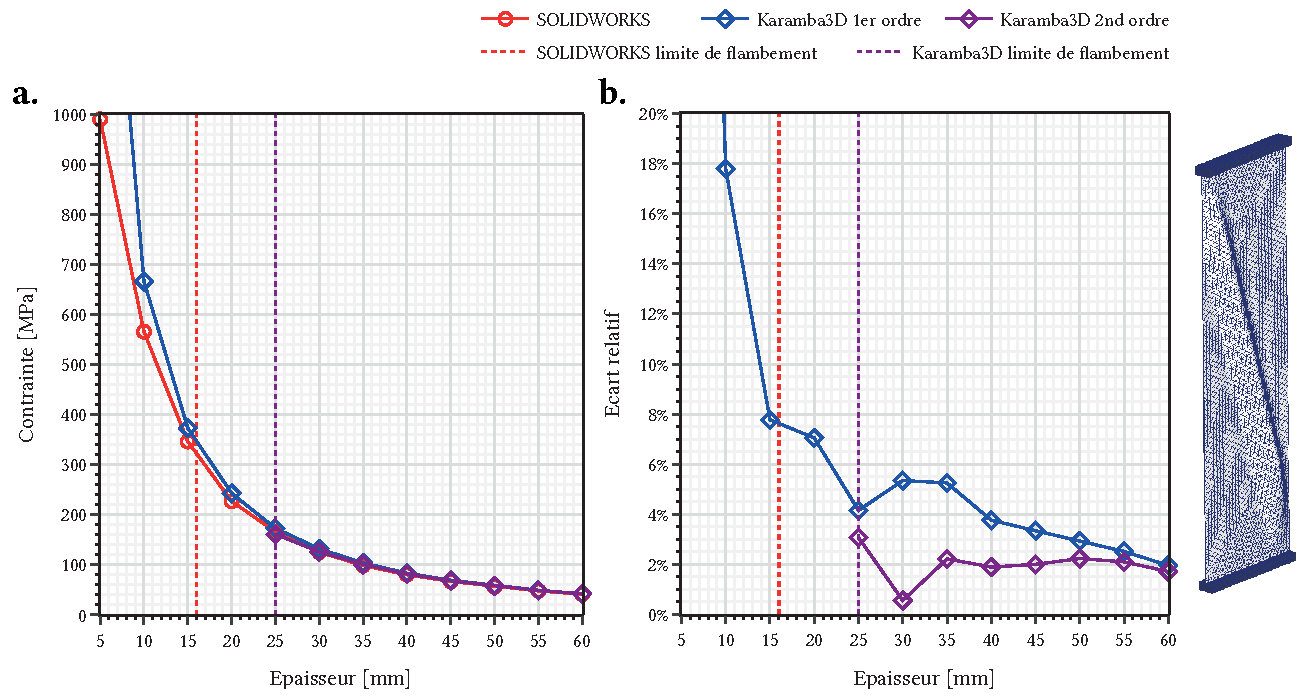
\includegraphics[width=\linewidth]{img/bulle/comp_kar.pdf}
    \caption{Comparaisons de la contrainte maximale calculée avec SOLIDWORKS et Karamba3D selon l'épaisseur de verre (\textbf{a.} contrainte maximale et \textbf{b.} écart relatif par rapport à SOLIDWORKS).}
    \label{fig:comp_kar}
\end{figure}

Pour chacunes des formes de bulles présentées dans la figure \ref{fig:types_bulle} on détermine, pour chaque épaisseur de verre, les meilleurs paramètres $h$ et $d$ afin de minimiser la quantité de verre sous contrainte de la résistance aux charges. On dresse dans la figure \ref{fig:surf_bulle} la surface minimale obtenue pour chacune des bulles.

\begin{figure}[H]
    \centering
    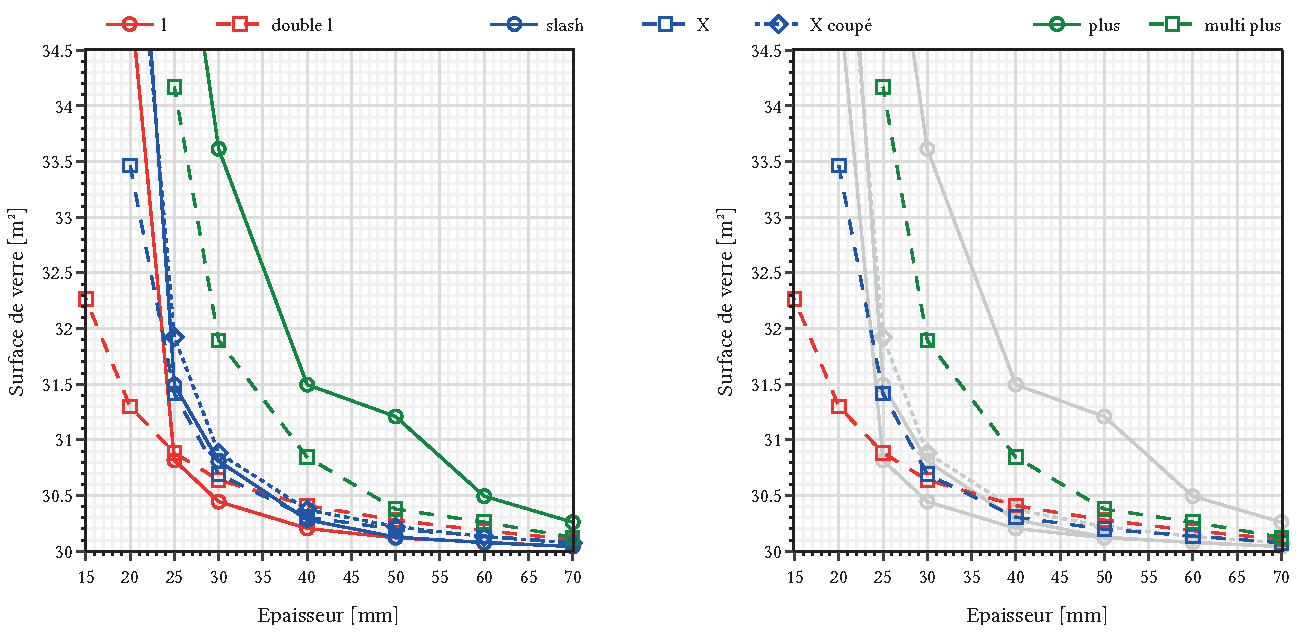
\includegraphics[width=\linewidth]{img/bulle/surf_bulle.pdf}
    \caption{Surface minimale selon l'épaisseur du verre pour chacunes des formes de bulles.}
    \label{fig:surf_bulle}
\end{figure}

On observe d'abord que pour toutes les formes, à l'exception du "double l", il n'est pas possible de trouver des valeurs de $h$ et $d$ permettant de résister aux charges lorsque l'épaisseur de verre est trop faible. Si l'on distingue les formes en trois groupes: les barres verticales ("l" et "double l"), les barres obliques ("slash","X" et "X coupé") et les croix ("plus" et "multi plus"), on peut alors déterminer dans chacun de ces groupes une forme plus optimale. Ce sont les formes "double l", "X" et "multi plus".

\begin{wrapfigure}{l}{0.4\textwidth}
    \centering
    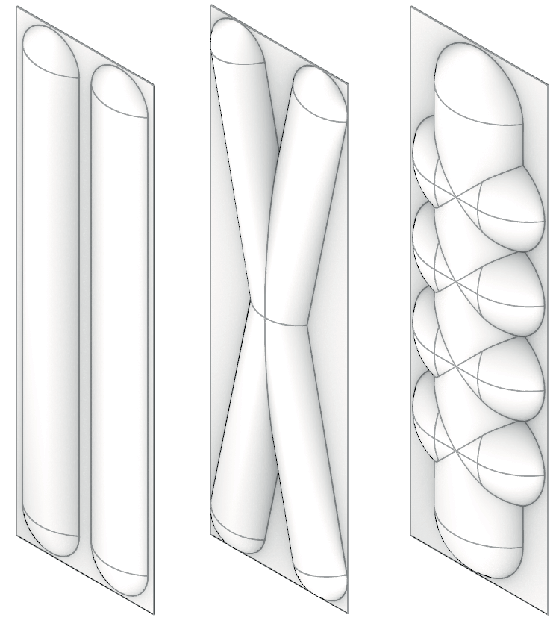
\includegraphics[width=\linewidth]{img/bulle/opti_bulle.pdf}
    \caption{Formes de bulles optimales}
    \label{fig:opti_bulle1}
    \vspace{-10pt}
    \end{wrapfigure}


\newpage
\subsection{Verre à double courbure}

\newpage

\section{Conclusions et perspectives}

\begin{table}[H]
    \centering
    \caption{Résultats finaux de l'optimisation.}
    \label{tab:result_fin}
    \begin{tabularx}{\textwidth}{l*{4}{Y}}
    \toprule
    \textbf{Solution} & \textbf{Plat}& \textbf{Cintrage simple} & \textbf{Ondulation}& \textbf{Bulle}\\\midrule
    \textbf{Épaisseur} [mm]& 71 / 57  & - & 22 / 16 & -  \\
    \textbf{Écart relatif} & - & - & \qty{69}{\percent} / \qty{72}{\percent} & - \\
    \textbf{Masse} [kg] & 5233 / 4201 & - & 1870 / 1115 & -  \\
    \textbf{Écart relatif} & - & - & \qty{64}{\percent} / \qty{68}{\percent} &  - \\
    \bottomrule
    \end{tabularx}
    \end{table}
\newpage
\begin{table}[H]
    \centering
    \caption{Résultats finaux de l'optimisation.}
    \label{tab:result_fin}
    \begin{tabularx}{\textwidth}{l*{4}{Y}}
    \toprule
    \textbf{Solution} & \textbf{Flat}& \textbf{Cold-bent} & \textbf{Wavy}& \textbf{Ribbed}\\\midrule
    \textbf{Thickness} [mm]& 71  & - & 22 & 10  \\
    \textbf{Relative difference} & - & - & \qty{69}{\percent}  & \qty{86}{\percent} \\
    \textbf{Weight} [kg] & 5233  & - & 1870 & 806 \\
    \textbf{Relative difference} & - & - & \qty{64}{\percent} &  \qty{85}{\percent} \\
    \bottomrule
    \end{tabularx}
    \end{table}
\newpage
\printbibliography

\end{document}